\documentclass[12pt,a4paper,boxed,titlepage]{caspset}

% set 1-inch margins in the document
%\usepackage[left=1in,right=1in,top=1.2in,bottom=1in]{geometry}
\usepackage[left=1in,right=1in,top=1.2in,bottom=1in]{geometry}
\usepackage{lastpage}
\usepackage{pdflscape}
% include this if you want to import graphics files with /includegraphics
\usepackage{graphicx}
\usepackage{lscape}
\usepackage{amsmath,amsfonts,amsthm,amssymb}
\usepackage{hyperref}
\usepackage{setspace}
\usepackage{fancyhdr}
\usepackage{lastpage}
\usepackage{extramarks}
\usepackage{chngpage}
\usepackage{soul}
\usepackage[usenames,dvipsnames]{color}
\usepackage{graphicx,float,wrapfig}
\usepackage{ifthen}
\usepackage{listings}
\usepackage{courier}
\usepackage{multimedia}
\usepackage[toc,page,title,titletoc,header]{appendix}
\usepackage{color, soul}
\usepackage{tikz}
\usepackage{array}
\usepackage{multirow}
\usepackage{todonotes}
\usepackage{pdfpages}
\usetikzlibrary{%
    decorations.pathreplacing,%
    decorations.pathmorphing,arrows
}
%%%%%%%%%%%%%%%%%%%%%%%%%%%%%%%%%%%%%%%%%%%%%%%%%%%%%%
\usepackage{xeCJK}
%\usepackage{fontspec}
\setCJKmainfont[BoldFont=simhei.ttf]{simsun.ttf}
\setCJKsansfont{simhei.ttf}
\setCJKmonofont{simfang.ttf}

%\setCJKmainfont{Adobe Song Std}
%\setCJKmainfont[BoldFont=Adobe Heiti Std]{Adobe Song Std}
%%%%%%%%%%%%%%%%%%%%%%%%%%%%%%%%%%%%%%%%%%%%%%%%%%%%%%

\graphicspath{{figures/}}

\setulcolor{red}

\setlength{\marginparwidth}{1in}

\newcommand{\hmwkTitle}{量纲分析}
%\newcommand{\hmwkSubTitle}{} % No subtitle, so this will be excluded
\newcommand{\hmwkDueDate}{\today}
\newcommand{\hmwkClass}{中科院力学所}
\newcommand{\hmwkClassTime}{Mon.{~}08:15}
\newcommand{\hmwkClassInstructor}{谈庆明}
\newcommand{\hmwkAuthorName}{周吕文}

\hypersetup{pdfauthor={\hmwkAuthorName}, 
            pdftitle={量纲分析作业整理}, 
            pdfsubject={\hmwkTitle, \hmwkClassInstructor},
            pdfkeywords={量纲分析, 力学},
            pdfproducer={XeLateX with hyperref},
            pdfcreator={Xelatex}}
%% Setup the header and footer
\pagestyle{fancy}                                                       %
\lhead{\hmwkAuthorName}                                                 %
\chead{\hmwkClass\ (\hmwkClassInstructor\ \hmwkClassTime): \hmwkTitle}  %
\rhead{第\ \thepage\ 页, 共\ \protect\pageref{LastPage} 页}          %



\makeatletter
\newcommand{\rmnum}[1]{\romannumeral #1}
\newcommand{\Rmnum}[1]{\expandafter\@slowromancap\romannumeral #1@}
\makeatother

\renewcommand\refname{\bf\large 参考文献}
\renewcommand\contentsname{\bf 目 \ \ \ 录}
\renewcommand\figurename{\bf 图}
\renewcommand\tablename{\bf 表}
\renewcommand{\appendixtocname}{附录}
\renewcommand{\appendixpagename}{附录}
\renewcommand\listfigurename{图目录}

% info for header block in upper right hand corner
%\name{周吕文{~}201128000718065}
%\class{物理学院{~}20110308班}
%\assignment{习题整理}
%\duedate{06/14/2014}

\newcommand\invisiblesection[1]{%
  \refstepcounter{section}%
  \addcontentsline{toc}{section}{\protect\numberline{\thesection}#1}%
  \sectionmark{#1}}

\newcommand\invisiblesubsection[1]{%
  \refstepcounter{subsection}%
  \addcontentsline{toc}{subsection}{\protect\numberline{\thesubsection}#1}%
  \subsectionmark{#1}}

\begin{document}
\title{量纲分析(2014春)习题整理\\ \vspace{-40pt} }

\author{{\Large 授课老师:谈庆明}\\ \vspace{50pt}\\ 周吕文\\ \href{mailto:zhou.lv.wen@gmail.com}{zhou.lv.wen@gmail.com}\\ \vspace{50pt}}
\date{中国科学院力学研究所\\2014年6月14日}
%\tableofcontents
\maketitle 
\enlargethispage{2\baselineskip}
\vspace{-0.5em}
\tableofcontents
\setcounter{page}{0}
\newpage

\invisiblesection{课前习题}
\problemlist{量纲分析{~}课前习题}
\invisiblesubsection{什么是量纲分析}
\begin{problem}[01]
什么是``量纲分析''?
\end{problem}
% --------------------------------------------------------------------
\begin{solution}
量纲分析就是在量纲法则(主要是$\Pi$定理)的原则下, 分析和探求物理量之间的关系. 量纲分析的精神实质:
\begin{itemize}
\item 只有同类量才能比较大小.
\item 物理现像和物理规律与所选用的度量单位无关.
\end{itemize}
具体说来: 量纲分析就是在控制某类物理现象或问题的物理量中, 先定一组物理量作为基本量, 并取作单位系统, 用以度量这类现象或问题中的任何物理量, 这样得到的该物理量的大小数值是无量纲的, 反映无量纲的因变量和自变量之间的因果关系, 也必然客观地反映这类现象的本质.
\end{solution}

\invisiblesubsection{为什么选修量纲分析}
\begin{problem}[02]
你为什么选修``量纲分析''课?
\end{problem}
% --------------------------------------------------------------------
\begin{solution}
我是刘谋斌研究员的学生, 现在主要研究方向是介观尺度下的微流动相关的数值模拟. 介观尺度不同于经典的连续介质力学, 它有一些由尺度效应引起的特殊现象, 因此想通过学习量纲分析来更好地理解和解释一些介观尺度的现象. 量纲分析的结论可以作为计算机模拟参数选择的参考, 以减少不必要的计算, 并对模拟结果做更深入的分析.
\end{solution}

\invisiblesubsection{流体是什么, 有什么性质}
\begin{problem}[03]
流体是什么, 有什么性质?
\end{problem}
% --------------------------------------------------------------------
\begin{solution}
流体的概念和性质分别如下:
\begin{itemize}
\item \textbf{流体}: 不能承受剪应力作用物体, 流体是一个理想的模型.
\item \textbf{性质}: 具有流动性, 没有确定形状, 流体不能承受切向力.
\end{itemize}
\end{solution}

\invisiblesubsection{什么是固体, 用什么来表征}
\begin{problem}[04]
什么是固体, 用什么来表征? (本构特征与状态参数)
\end{problem}
% --------------------------------------------------------------------
\begin{solution}
固体是具有固定的体积及形状, 能承受剪切的宏观物体, 固体也是理想化模型. 固体用位移描述(与之对应的, 流体用速度描述), 固体材料在受到应力作用时, 会引起形状变化,和其原有形状不同,称为形变,形变和原有尺寸的比例称为应变. 线弹性材料的形变与外加的载荷成正比. 弹性固体材料性质由杨氏模量和泊松比描述.
\end{solution}

\newpage
\invisiblesubsection{怎样表征固体的弹塑性}
\begin{problem}[05]
怎样表征固体的弹塑性, 有何重要特点?
\end{problem}
% --------------------------------------------------------------------
\begin{solution}
在弹性阶段(材料受应力较小), 当外力移除后,物体会恢复成原来形变前的状态. 当外力造成的应力超过一定范围时, 物体会产生不可逆的永久形变, 外力移除后,物体无法完全恢复成原来的状态, 称为弹塑性变形. 固体的弹塑性可由应力-应变曲线及屈服点描述: 
\begin{itemize}
\item 屈服点前是弹性变形, 应力-应变程线性关系, 可逆; 
\item 屈服点后是弹塑性变形, 应力-应变程非线性关系, 不可逆.
\end{itemize}
\end{solution}

\invisiblesubsection{什么是耦合}
\begin{problem}[06]
什么是耦合?
\end{problem}
% --------------------------------------------------------------------
\begin{solution}
耦合是指两种或多种现象或系统的交互作用.
\end{solution}

\invisiblesubsection{什么是动态/静态/准静态}
\begin{problem}[07]
什么是动态(动力学), 静态(静力学), 准静态.
\end{problem}
% --------------------------------------------------------------------
\begin{solution}
\begin{itemize}
\item \textbf{动\hphantom{动}态}: 非平衡的问题是动力学或动态问题.
\item \textbf{静\hphantom{静}态}: 平衡的问题是静力学或静态问题.
\item \textbf{准静态}: 准静态是指动态过程可看成无限多个变化非常慢的过程的组合, 这要求系统发生的变化无限慢.
\end{itemize}
\end{solution}


\newpage

\invisiblesection{课后习题}
\problemlist{量纲分析{~}课后习题}
\invisiblesubsection{量纲与单位的区别和关系}
\begin{problem}[01]
量纲是否就是单位, 两者之间有什么关系?
\end{problem}
% --------------------------------------------------------------------
\begin{solution}
量纲不是单位, 单位与量纲密切相关, 但内含的概念大不相同:
\begin{itemize}
\item \textbf{量纲}是用来表示物理量的本质属性, 而不表示该量的大小. 不同属性的物理量具有不同的量纲, 任何相同属性的物理量都有唯一相同的量纲, 这与单位无关.
\item \textbf{单位}是用来表示物理量数量大小的标准量, 同一个物理量可以选用不同的单位, 不同单位之间可以相互转化, 一个物理量的数值大小与所选用的度量单位有关.
\end{itemize}
量纲(物理性质)不同的量作比较是没有意义的, 只有具有相同量纲(物理性质)的物理量, 才能正确的进行比较. 
\end{solution}

\invisiblesubsection{Dimension词义和演变}
\begin{problem}[02]
``Dimension''一词包含什么函义? 说说它的历史演变.
\end{problem}
% --------------------------------------------------------------------
\begin{solution}
\begin{itemize}
\item 有道词典给出``Dimension''作为名词的\textbf{主要函义}\cite{youdao_dimension}: 1. [数学]维(数), 维数度, 因次; 2. 尺寸, 长度; 宽度; 厚度; 深度; 3. 面积, 大小; 容积, 体积; 量; 4. [物理]量纲.
\item \textbf{历史演变}: 始有``维数''的意思; 再有``长度, 尺寸''的意思, 指运动学, 几何学上的概念; 后有物理维度的意思;  后来出现``量纲''的函义, 用来表示物理量的本质属性.
\end{itemize}
\end{solution}

\invisiblesubsection{自由落体的提法}
\begin{problem}[03]
自由落体问题有哪几种提法? 各有哪些基本量和导出量?
\end{problem}
% --------------------------------------------------------------------

\begin{solution}
\begin{minipage}[c]{0.8\linewidth}
自由落体问题涉及的物理量有高度$h$, 重力加速度$g$, 下落时间$t$. 可取任意两个量为基本量, 另一量为导出量, 因此自由落体问题有以下三种提法:
\begin{itemize}
\item 已知$h$, $g$, 求$t$. 以$h$, $g$为基本量, $t$为导出量: $t = f(h,g)$.
\item 已知$g$, $t$, 求$h$. 以$g$, $t$为基本量, $h$为导出量: $h = f(g,t)$.
\item 已知$h$, $t$, 求$t$. 以$h$, $t$为基本量, $g$为导出量: $g = f(h,t)$.
\end{itemize}
\end{minipage}
\begin{minipage}[c]{0.2\linewidth}
\begin{center}
\usetikzlibrary{%
    decorations.pathreplacing,%
    decorations.pathmorphing,arrows
}
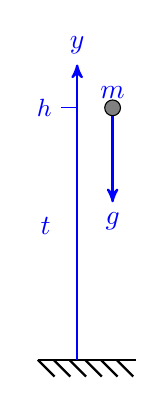
\begin{tikzpicture}[ media/.style={font={\footnotesize\sffamily}},
    wave/.style={
        decorate,decoration={snake,post length=1.4mm,amplitude=2mm,
        segment length=2mm},thick},
    interface/.style={
        postaction={draw,decorate,decoration={border,angle=-45,
                    amplitude=0.3cm,segment length=2mm}}}]
\draw[thick,interface](-0.5,0)--(0.75,0);
\draw[ ->,>=stealth',thick,blue](0,0) -- (0,3.75) node[above]{$y$};

\draw[blue] (0,3.2)--(-.2,3.2) node[left,blue]{\small $h$};
\draw [blue,->,>=stealth',thick] (0.45,3.2) -- (0.45, 2) node [below]{$g$};
\draw [fill=gray](0.45,3.2) circle(0.1) node [above,blue]{$m$};
\node[blue] at (-0.4, 1.7) {$t$};
\end{tikzpicture}
\end{center}
\end{minipage}
\end{solution}

\invisiblesubsection{摆锤质量与单摆周期无关的原因}
\begin{problem}[04]
从物理上分析摆锤质量与单摆周期无关的原因.
\end{problem}
% --------------------------------------------------------------------
\begin{solution}
\begin{minipage}[c]{0.8\linewidth}
\begin{itemize}
\item \textbf{证明}: 对于如右图所示的单摆, 摆长为$l$, 选取自然坐标系, 摆锤的的位置可由弧长$s=l\theta$确定, 摆锤受到的合力沿垂直于摆长的方向, 大小为$f = mg\sin\theta$, 因此摆锤加速度$a$为
\[
a = \frac{f}{m} = g\sin\theta = \frac{d^2s}{dt^2} = l\frac{d^2\theta}{dt^2}
\quad \Longrightarrow \quad \ddot{\theta} -\frac{g}{l}\sin\theta = 0
\]
显然上式最终得到的运动学方程中不含摆锤质量, 可见摆锤质量与单摆周期无关.
\end{itemize}
\end{minipage}
\begin{minipage}[c]{0.2\linewidth}
\begin{center}
\usetikzlibrary{%
    decorations.pathreplacing,%
    decorations.pathmorphing,arrows
}
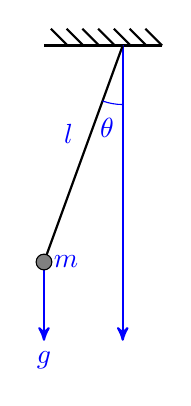
\begin{tikzpicture}[ media/.style={font={\footnotesize\sffamily}},
    wave/.style={
        decorate,decoration={snake,post length=1.4mm,amplitude=2mm,
        segment length=2mm},thick},
    interface/.style={
        postaction={draw,decorate,decoration={border,angle=-45,
                    amplitude=0.3cm,segment length=2mm}}}]
\draw[thick,interface] (0.5,3.75)--(-1,3.75);
\draw[->,>=stealth',thick,blue](0,3.75)--(0,0);

\draw [thick](0,3.75)--(-1,1) node[midway,above left,blue]{$l$};
\draw [blue,->,>=stealth',thick] (-1,1) -- (-1, 0) node [below]{$g$};
\draw [fill=gray](-1,1) circle(0.1) node [right,blue]{$m$};
\draw[blue] (0,3) arc(-90:-110:0.75);
 \node[blue] at (-0.2,2.7) {$\theta$};
\end{tikzpicture}
\end{center}
\end{minipage}
\begin{itemize}
\item \textbf{分析}: 摆锤的运动完全由重力加速度决定, 摆锤的运动是一个纯运动学的问题, 与质量无关, 所以摆锤质量与单摆周期无关, 因此\textbf{上述证明可以直接不引入质量}.
\end{itemize}
\end{solution}

\invisiblesubsection{谐振子的自振频率}
\begin{problem}[05]
求谐振子的自振频率.
\end{problem}
% --------------------------------------------------------------------
\begin{solution}
\begin{minipage}[c]{0.8\linewidth}
如右图所示, 谐振子的自振频率$f$仅与弹簧的弹性系数$k$及振子的质量$m$有关. 因此
\[
f = g(m,k)
\]
\end{minipage}
\begin{minipage}[c]{0.2\linewidth}
\begin{center}
\usetikzlibrary{%
    decorations.pathreplacing,%
    decorations.pathmorphing,arrows
}
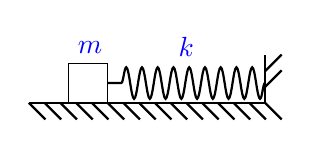
\begin{tikzpicture}[ media/.style={font={\footnotesize\sffamily}},
    wave/.style={
        decorate,decoration={snake,post length=1.4mm,amplitude=2mm,
        segment length=2mm},thick},
    interface/.style={
        postaction={draw,decorate,decoration={border,angle=-45,
                    amplitude=0.3cm,segment length=2mm}}}]
\draw[thick,interface](0,0)--(3,0)--(3,0.6);
\draw[wave](3,0.25)--(1,0.25) node[above=6pt,midway,blue]{$k$};
\draw  (1,0) rectangle (0.5,0.5) node[above right,blue]{$m$};

\end{tikzpicture}
\end{center}
\end{minipage}
上式中各物理量的量纲分别为: $[f] = T^{-1}$, $[m]=M$, $[k] = MT^{-2}$, 以$m$, $k$为基本量并作为单位, 有
\[
\frac{f}{\sqrt{k/m}} = g\bigg(\frac{m}{m},\frac{k}{k}\bigg) = g(1,1) = C
\]
其中$C$为常数, 因此谐振子的自振频率为: $f = C\sqrt{k/m}$. 理论上可得$C=2\pi$.
\end{solution}

\invisiblesubsection{由偏导数关系推导量纲函数的最终表示式}
\begin{problem}[06]
从量纲幂次式的讨论中得到的偏导数关系, 求出量纲函数的最终表示式.
\end{problem}
% --------------------------------------------------------------------
\begin{solution}
书\cite{tan_dimensional_2011}中式(2.10)为从量纲幂次式的讨论中得到的偏导数关系, 即以下三式:
\[
\frac{\frac{\partial f}{\partial r_l}(r_l, r_m, r_t)}{f(r_l, r_m, r_t)} = \frac{\alpha}{r_l}
, \qquad
\frac{\frac{\partial f}{\partial r_m}(r_l, r_m, r_t)}{f(r_l, r_m, r_t)} = \frac{\beta}{r_m}
, \qquad
\frac{\frac{\partial f}{\partial r_t}(r_l, r_m, r_t)}{f(r_l, r_m, r_t)} = \frac{\gamma}{r_t}
\]
整理上式, 并将$f(r_l, r_m, r_t)$简写为$f$可得
\begin{equation}\label{eq:partialF/partialR}
\frac{\partial f}{\partial r_l}= \frac{\alpha}{r_l}f
, \qquad
\frac{\partial f}{\partial r_m}= \frac{\beta}{r_m}f
, \qquad
\frac{\partial f}{\partial r_t}= \frac{\gamma}{r_t}f
\end{equation}
对函数$f(r_l, r_m, r_t)$进行全微分得
\begin{equation}\label{eq:df}
df = \frac{\partial f}{\partial r_l}dr_l + \frac{\partial f}{\partial r_m}dr_m + \frac{\partial f}{\partial r_t}dr_t
\end{equation}
将式(\ref{eq:partialF/partialR})代入式(\ref{eq:df})得
\begin{equation}
df = \alpha f \frac{dr_l}{r_l} + \beta f \frac{dr_m}{r_m} + \gamma f \frac{dr_t}{r_t} 
\quad \Longrightarrow \quad 
\frac{df}{f} = \alpha \frac{dr_l}{r_l} + \beta \frac{dr_m}{r_m} + \gamma \frac{dr_t}{r_t}
\end{equation}
对上式得到的关系两边同时进行积分得
\begin{equation}
\ln f = \alpha \ln r_l + \beta \ln r_m + \gamma \ln r_t + \ln C
\quad \Longrightarrow \quad 
f = C r_r^{\alpha} r_m^{\beta} r_t^{\gamma}
\end{equation}
其中$C$为待定常数, 若单位系中的长度, 质量, 和时间不变, 则对应的缩放倍数可看成$r_l=1$, $r_m=1$, $r_t=1$, 显然有$f(1,1,1) = C = 1$. 因此
\begin{equation}
f = r_r^{\alpha} r_m^{\beta} r_t^{\gamma}
\end{equation}
可见, 与之相对应, 物理量$X$的量纲表达式应为
\[
[X] = L^\alpha M^\beta T^\gamma
\]
\end{solution}

\newpage
\invisiblesubsection{相似三定理与$\Pi$定理}
\begin{problem}[07]
查阅基尔比契夫提出的``相似三定理''说的是什么? 它与$\Pi$定理的说法不同, 哪种说法更为本质?
\end{problem}
% --------------------------------------------------------------------
\begin{solution}
基尔比契夫提出的``相似三定理''可分别表述如下\cite{zlvo3}:
\begin{itemize}
\item \textbf{相似第一定理}: 彼此相似的现象, 其同名相似准则的数值相同.
\item \textbf{相似第二定理}: 物理现象中各物理量之间的关系, 可以化为各相似准则之间的关系.
\item \textbf{相似第三定理}: 如果两个现象的单值条件相似, 而且由单值量组成的同名相似准则数值相同, 则这两个现象相似.
\end{itemize}
而$\Pi$定理可概括为:
\begin{itemize}
\item \textbf{$\Pi$定理}: 问题中若有$N$个变量, 即$n$个自变量$a_1,a_2,\cdots a_n$和应变量$a$, 那么因变量$a$可表示为自变量的函数$a=f(a_1,a_2,\cdots, a_n)$, 而基本量的数目是$k$, 那么一定形成$N-k$个无量纲量, 即1个无量纲应变量$\Pi$和$n-k$个无量纲自变量$\Pi_1,\Pi_2,\cdots, \Pi_{n-k}$, 它们之间形成确定的函数关系$\Pi = F(\Pi_1,\Pi_2,\cdots, \Pi_{n-k})$.
\end{itemize}
基尔比契夫提出的``相似三定理''与$\Pi$定理相比, 显然$\Pi$定理更为简单, 两者表述中相对应的关系如下:
\begin{itemize}
\item $\Pi$定理中的``变量''对应相似三定理表述中的``物理量'';
\item $\Pi$定理中的``无量纲量''对应相似三定理表述中的``同名相似准则'';
\item 显然$\Pi$定理中, 对同一个函数$F$, 各无量纲量值相同时, $F$的值也必定唯一, 这对应相似三定理表述中的``单值条件相似''.
\end{itemize}
与相似三定理相比, $\Pi$定理也更为本质. $\Pi$定理包含了相似三定理: 
\begin{itemize}
\item \textbf{相似第一定理}: 若两个物理现象具有相同的函数关系$\Pi = F(\Pi_1,\Pi_2,\cdots, \Pi_{n-k})$, 则其无量纲量数值相同.
\item \textbf{相似第二定理}: 物理现象中的$N=n+1$个变量间的关系$a=f(a_1,a_2,\cdots, a_n)$, 可以化为无量纲量间的函数关系$\Pi = F(\Pi_1,\Pi_2,\cdots, \Pi_{n-k})$.
\item \textbf{相似第三定理}: 若两物理现象中各无量纲量$\Pi_1,\Pi_2,\cdots,\Pi_{N-k}$数值相等, 且函数$F$关系相同, 则$\Pi = F(\Pi_1,\Pi_2,\cdots, \Pi_{n-k})$的函数值也必定单值唯一.
\end{itemize}
\end{solution}

\newpage
\invisiblesubsection{隐函数法证明$\Pi$定理}
\begin{problem}[08]
用隐函数法证明$\Pi$定理.
\end{problem}
% --------------------------------------------------------------------
\begin{solution}
把物理问题的因变量和自变量都统一视作变量, 若其总数为$N$, 并分别记为$a_1,a_2,\cdots,a_N$, 那么物理规律可表示为以下隐函数关系:
\[
f(a_1, a_2, \cdots, a_N) = 0
\]
在上式涉及到的$N$个变量中, 选出$k$个基本量, 不妨排在前面, 它们是$a_1,a_2,\cdots,a_k$, 其量纲分别为$A_1, A_2, \cdots, A_k$. 而后面$N-k$个变量则是导出量, 其量纲可表示为基本量的量纲的幂次式:
\begin{align*}
[a_{k+1}] & =A_{1}^{p_{1}}A_{2}^{p_{2}}\cdots A_{k}^{p_{k}}\\{}
[a_{k+2}] & =A_{1}^{q_{1}}A_{2}^{q_{2}}\cdots A_{k}^{q_{k}}\\
& \vdots\\{}
[a_{N}] & =A_{1}^{t_{1}}A_{2}^{t_{2}}\cdots A_{k}^{t_{k}}
\end{align*}
用$k$个基本量单位系统来度量函数关系中的各变量, 由此得到以下关系
\[
f\Bigg(\underbrace{1,\cdots,1}_{k\text{个}},\frac{a_{k+1}}{a_{1}^{p_{1}}a_{2}^{p_{2}}\cdots a_{k}^{p_{k}}},\; \frac{a_{k+2}}{a_{1}^{q_{1}}a_{2}^{q_{2}}\cdots a_{k}^{q_{k}}},\cdots\frac{a_{N}}{a_{1}^{t_{1}}a_{2}^{t_{2}}\cdots a_{k}^{t_{k}}}\Bigg)=0
\]
上式中对函数$f$起作用的变量仅为后面的$N-k$个无量纲变量, 分别记为$\Pi_1,\Pi_2,\cdots, \Pi_{N-k}$, 则上式可表示为
\[
f(\Pi_1,\Pi_2,\cdots, \Pi_{N-k})=0
\]
\end{solution}

\invisiblesubsection{小孔出流速度}
\begin{problem}[09]
求盛水容器底侧的小孔出流速度.
\end{problem}
% --------------------------------------------------------------------
\begin{solution}
\begin{minipage}[c]{0.8\linewidth}
小孔出流是一个纯粹的力学问题, 与容器中水的高度$h$, 重力加速度$g$和小孔的直径$d$有关, 小孔出流速度为$v$, 则有
\[
v = f(d, g, h)
\]
\end{minipage}
\begin{minipage}[c]{0.2\linewidth}
\begin{center}
\usetikzlibrary{%
    decorations.pathreplacing,%
    decorations.pathmorphing,arrows
}
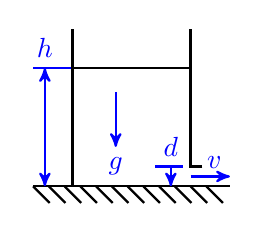
\begin{tikzpicture}[ media/.style={font={\footnotesize\sffamily}},
    wave/.style={
        decorate,decoration={snake,post length=1.4mm,amplitude=2mm,
        segment length=2mm},thick},
    interface/.style={
        postaction={draw,decorate,decoration={border,angle=-45,
                    amplitude=0.3cm,segment length=2mm}}}]
\draw[thick,interface](-1.25,0)--(1.25,0);
\draw[thick] (-0.75,0) -- (-0.75,2);
\draw[thick] (0.9,0.25)--(0.75,0.25) -- (0.75,2);

\draw[thick,->,>=stealth',blue] (0.75,0.125)--(1.25,0.125) node[above left=-1pt]{$v$};

\draw[thick](-0.75,1.5)--(0.75,1.5);
\draw[thick,blue](-0.77,1.5)--(-1.25,1.5);
\draw[ <->,>=stealth',thick,blue](-1.1,0) -- (-1.1,1.5) node[above]{$h$};

\draw[thick,blue](0.3,0.25) -- (0.65,0.25);
\draw[ <-,>=stealth',thick,blue](0.5,0) -- (0.5,0.25) node[above]{$d$};


\draw [blue,->,>=stealth',thick] (-0.2,1.2) -- (-0.2, 0.5) node [below]{$g$};
\end{tikzpicture}
\end{center}
\end{minipage}
上式中各物理量的量纲分别为:$[v]=LT^{-1}$, $[d]=L$, $[g]=LT^{-2}$, $[h]=L$, 取$h,g$为基本量, 且作为本问题的单位系统, 用以度量问题中的各量, 于是上式转化为
\[
\frac{v}{\sqrt{gh}}=f\bigg(\frac{d}{h},1,1\bigg)=f\bigg(\frac{d}{h}\bigg)
\]
由于小孔有$d\ll h$, 则有$d/h\rightarrow 0$, 所以$f(d/h)=f(0)=C$, 因此小孔出流速度为
\[
v = C\sqrt{gh}
\]
其中$C$为常数, 可进一步由理论确定$C=\sqrt{2}$.
\end{solution}

\newpage
\invisiblesubsection{三角形断面的溢洪流量}
\begin{problem}[10]
若溢洪道的断面为三角形, 讨论溢洪流量.
\end{problem}
% --------------------------------------------------------------------
\begin{solution}
\begin{minipage}[c]{0.8\linewidth}
溢洪流量与流体的密度$\rho$, 重力加速度$g$, 上游水头$h$及三角形的顶角$\alpha$有关, 溢过三角形断面的流量为$Q$, 则有
\[
Q = f(\rho, g, h, \alpha)
\]
\end{minipage}
\begin{minipage}[c]{0.2\linewidth}
\begin{center}
\usetikzlibrary{calc,intersections,through,backgrounds}
\usetikzlibrary{decorations.pathreplacing,decorations.pathmorphing,arrows}
\begin{tikzpicture}
\coordinate (p1) at (0.6,0.2);
\coordinate (p2) at  (1.2,0.4);
\coordinate (p4) at (2,-0.2);
\coordinate (p6temp) at (2.5,1);
\coordinate (p7) at (3,1);
\path [name path=D] (p1)--(3,1);
\path [name path=E] (p4)--(p6temp);
\path [name intersections={of=D and E, by=p6}];

\coordinate (pd1) at (0,-0.4);
\path [name path=A] (pd1)--(3.9,0.9);
\path [name path=B] (p2)--(p4);
\path [name intersections={of=A and B, by=p3}];
\path [name intersections={of=A and E, by=p5}];

\draw[thick] (p1) -- (p2)--(p3)--(p4)  (p5)-- (p6)--(p7);
\draw[dashed, thick] (p4)--(p5);

\draw[dashed, thick] (p1)++(0,-0.4)--(p3) (p7)++(0,-0.4) -- (p5);

\draw[thick](p1)++(0,-0.9)--(p4);

\node at (1.55,0.125) {\includegraphics[width=60pt]{water.pdf}};
\draw[ <->,>=stealth',thick,blue](1,-0.09) -- (1,-0.55) node[right=-1pt, midway]{$h$};
\draw[ <->,>=stealth',thick,blue](p5) arc(80:138:0.707);
\node[blue] at (1.8,0.5) {$\alpha$};
\node[blue] at (1.25,1) {$\rho$};
\node[blue] at (2.0,-0.75) {$Q$};
\draw [blue,->,>=stealth',thick] (3,0.25) -- (3, -0.5) node [below]{$g$};
\end{tikzpicture}

\end{center}
\end{minipage}
上式中的各物理量的量纲分别为: $[Q]=MT^{-1}$, $[\rho]=ML^{-3}$, $[g]=LT^{-2}$, $[h]=L$, 而$\alpha$为无量纲量. 选取$\rho$, $g$, $h$三个量作为基本量, 且作为本问题的单位系统, 用以度量问题中的各量. 于是, 得到各量的量值所满足的关系
\[
\frac{Q}{\rho h^3 \sqrt{g/h}} = f(1,1,1,\alpha) \qquad \Longrightarrow \qquad Q = \rho g^{1/2} h^{5/2}f(\alpha)
\]
\end{solution}


\invisiblesubsection{定常管流的摩擦系数}
\begin{problem}[11]
分析定常管流问题中的摩擦系数; 什么情况下可不考虑密度的影响? 说明其物理原因.
\end{problem}
% --------------------------------------------------------------------
\begin{solution}
\begin{minipage}[c]{0.8\linewidth}
摩擦系数$c_d$可以用单位面积摩擦力与动压之比定义. 因此摩擦系数$c_d$与管径$d$, 流体密度$\rho$, 平均流速$v$, 粘性系数$\mu$有关:
\[
c_d = f(d,\rho, v, \mu)
\]
\end{minipage}
\begin{minipage}[c]{0.2\linewidth}
\begin{center}
\usetikzlibrary{calc,intersections,through,backgrounds}
\usetikzlibrary{decorations.pathreplacing,decorations.pathmorphing,arrows}
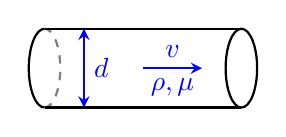
\begin{tikzpicture}
	\draw[dashed,color=gray, thick] (0,0) arc (-90:90:0.2 and 0.5);% right half of the left ellipse
	\draw[thick] (0,0) -- (2.5,0);% bottom line
	\draw[thick] (0,1) -- (2.5,1);% top line
	\draw[thick] (0,0) arc (270:90:0.2 and 0.5);% left half of the left ellipse
	\draw[thick] (2.5,0.5) ellipse (0.2 and 0.5);% right ellipse
    \draw[<->, >=stealth, thick,blue](0.5,0)--(0.5,1) node[right,midway] {$d$};
    \draw[->, >=stealth, thick,blue](1.25,0.5)--(2,0.5) node[above,midway] {$v$} node[below, midway]{$\rho, \mu$};
\end{tikzpicture}
\end{center}
\end{minipage}
上式中各物理量的量纲分别为: $c_d$为无量纲量, $[d]=L$, $[\rho]=ML^{-3}$, $[v]=LT^{-1}$, $[\mu]=ML^{-1}T^{-1}$. 取$\rho$, $v$, $d$为基本量, 且作为本问题的单位系统, 用以度量问题中的各量, 于是上式转化为
\[
c_d = f\bigg(1,1,1,\frac{\mu}{\rho v d}\bigg) = f\bigg(\frac{\rho v d}{\mu}\bigg)=f(\mathrm{Re})
=f\bigg(\frac{\rho}{\mu/(vd)}\bigg)\]
显然当雷诺数$\mathrm{Re}=\frac{\rho}{\mu/(vd)}$较小时, 可不考虑密度. 雷诺数$\mathrm{Re}$较小时, 流动为层流, 流体中的每个质点都做匀速运动, 相对于粘性力, 流体受惯性力影响较小, 因此这种情况下可以不考虑惯性即密度的影响.
\end{solution}

\invisiblesubsection{水洞/风洞做机翼/潜艇的模型实验}
\begin{problem}[12]
能否用水洞做机翼的模型实验, 或用风洞做潜艇的模型实验? 如果可以, 问尺寸和速度的缩比范围?
\end{problem}
% --------------------------------------------------------------------
\begin{solution}

\noindent\begin{minipage}[c]{0.7\linewidth}
先不具体讨论机翼或潜艇, 统称为固体, 假设固体形状的特征长度是$l, l', \cdots$, 均匀来流速度为$v$, 方位角为$\alpha$, 流体的密度为$\rho$, 粘性系数为$\mu$. 则固体受到流体的作用力$W$可表示为
\end{minipage}
\begin{minipage}[c]{0.3\linewidth}
\begin{center}
%\usetikzlibrary{calc,intersections,through,backgrounds}
\usetikzlibrary{decorations.pathreplacing,decorations.pathmorphing,arrows}
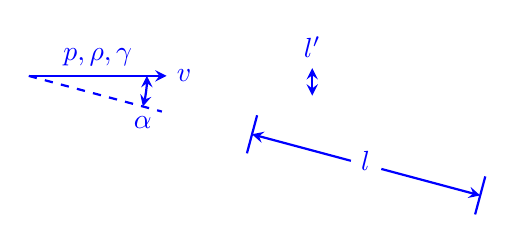
\begin{tikzpicture}
        % Some profiles look better when using plot[smooth]
        \draw[scale=3, rotate=-15, thick]
            plot file{./figures/airfoil.dat} -- cycle;
    \draw[thick,blue] (-0.1,-0.5)--++(-105:0.5) (-0.1,-0.5)++(-15:3)--++(-105:0.5);
	\draw[<-,thick, >=stealth,blue] (-0.1,-0.5)++(-105:0.25) -- ++(-15:1.3) node[right]{$l$};
	\draw[->,thick, >=stealth,blue] (-0.1,-0.5)++(-105:0.25) ++(-15:1.7)--++(-15:1.3);

\draw [->,thick, blue, >=stealth](-3,0)--(-1.25,0) node[right] {$v$} node[above,midway] {$p, \rho, \gamma$}; 
\draw [thick, blue, >=stealth,dashed](-3,0)--++(-15:1.75);
\draw [<->,thick, blue, >=stealth](-1.5,0) arc(0:-15:1.5) node[below] {$\alpha$};
\draw[<->,thick,blue,>=stealth] (0.6,-0.25)--(0.6,0.1) node[above] {$l'$};
\end{tikzpicture}
\usetikzlibrary{%
    decorations.pathreplacing,%
    decorations.pathmorphing,arrows
}

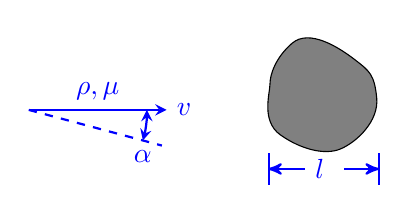
\begin{tikzpicture}


\draw [->,thick, blue, >=stealth](-3,0.85)--(-1.25,0.85) node[right] {$v$} node[above,midway] {$\rho, \mu$}; 
\draw [thick, blue, >=stealth,dashed](-3,0.85)--++(-15:1.75);
\draw [<->,thick, blue, >=stealth](-1.5,0.85) arc(0:-15:1.5) node[below] {$\alpha$};

\begin{scope}[y=0.80pt, x=0.8pt,yscale=-1,yshift=-850]
  \path[draw=black,fill=gray] (12.2092,1002.1870) .. controls (4.7404,1008.6595) and
    (2.2567,1016.3308) .. (2.2567,1020.5208) .. controls (2.2567,1024.7120) and
    (-1.9333,1037.2845) .. (6.9717,1043.5708) .. controls (15.8767,1049.8570) and
    (26.8779,1053.0008) .. (34.2117,1049.8570) .. controls (41.5467,1046.7145) and
    (51.4992,1037.2845) .. (50.4517,1026.8083) .. controls (49.4042,1016.3308) and
    (47.3079,1014.7595) .. (40.4967,1009.5208) .. controls (33.6892,1004.2820) and
    (20.0679,995.3758) .. (12.2092,1002.1870) -- cycle;
\end{scope}

\draw[thick,blue] (0.05,-0.1)--(0.05,0.3) (1.45,-0.1)--(1.45,0.3);
\draw[thick,blue,<-,>=stealth'](0.04,0.1)--(0.51,0.1) node[right] {$l$};
\draw[thick,blue,<-,>=stealth'](1.45,0.1)--(1.0,0.1);
\end{tikzpicture}

\end{center}
\end{minipage}
\[
W = f(l,l',\cdots, v, \alpha; \rho, \mu)
\]
上式中各物理量的量纲分别为:$[l]=[l']=\cdots=L$, $[v]=LT^{-1}$, $\alpha$为无量纲量, $[\rho]=ML^{-3}$, $[\mu]=ML^{-1}T^{-1}$. 选取$l$, $v$, $\rho$作为基本量, 且作为本问题的单位系统, 用以度量问题中的各量. 于是, 得到各量的量值所满足的关系
\[
\frac{W}{\rho v^2 l^2} = f\bigg(1,\frac{l'}{l},\cdots,\alpha,1,\frac{\mu}{\rho vl}\bigg) 
\quad\Longrightarrow\quad
 W = \rho v^2 l^2 f(l'/l,\cdots,\alpha,\mathrm{Re})
\]
如果要用模型实验来求取无量纲函数$f$, 那么在模型(用下标$\mathrm{m}$表示)和原型(用下标$\mathrm{p}$表示)之间, 要满足以下两方面条件
\begin{itemize}
\item 几何相似: $(l'/l,\cdots)_\mathrm{m}=(l'/l,\cdots)_\mathrm{p}$ 及 $\alpha_m = \alpha_p$
\item 动力学相似: $(\mathrm{Re})_\mathrm{m} = (\mathrm{Re})_\mathrm{p}$
\end{itemize}
基于上面对一般情况的分析, 下面分别讨论水洞做机翼的模型实验和风洞做潜艇的模型实验的可行性:
\begin{enumerate}
\item \textbf{水洞做机翼的模型实验:}

世界上最大的水洞一般认为是宾夕法尼亚州立大学的Garfield Thomas水洞\cite{Garfield,wiki_Water_tunnel}, 长$30\mathrm{m}$, 高达$10\mathrm{m}$, 最大水流速度可达$18\mathrm{m/s}$. 而超高速的水洞来流速度可达$84\mathrm{m/s}$\cite{Garfield}. 对于一般的水洞(本题中所考虑的水洞), 直径通常小于$2\mathrm{m}$, 来流速度小于$10\mathrm{m/s}$. 
美国比较流行的CTSW私人小飞机\cite{CTSW}其翼展为$8.5\mathrm{m}$, 全长$6.2\mathrm{m}$, 总高$2.2\mathrm{m}$, 最低巡航速度$65\mathrm{km/h}$. 本题飞机的参数选取主要参考CTSW私人小飞机.
\begin{figure}[!htb]
\centering
\begin{minipage}[t]{.495\linewidth}
\centering
\usetikzlibrary{%
    decorations.pathreplacing,%
    decorations.pathmorphing,arrows
}

\definecolor{ca5bed6}{RGB}{210,210,210}
\definecolor{c1a232b}{RGB}{80,80,80}
\definecolor{c2c3c57}{RGB}{100,100,100}
\definecolor{c354b6b}{RGB}{130,130,130}
\definecolor{c453f41}{RGB}{120,120,120}
\definecolor{caed0e3}{RGB}{250,250,250}
\definecolor{cffffff}{RGB}{255,255,255}


\begin{tikzpicture}[
 interface/.style={
        postaction={draw,decorate,decoration={border,angle=-45,
                    amplitude=0.3cm,segment length=2mm}}}]
\node[blue] at (1.25,-2.5) {Water Tunnel};
\node[black!80] at (1.25,0.15) {Model};
\node[red] at (2.5,-1.5) {Struct};

\draw[thick,interface,blue] (4,0.75)--(-1.5,0.75)  (-1.5,-2)--(4,-2)  ;
\draw[semithick,fill=red!30,draw=red,rounded corners=1](2.8,-0.625)--(3.2,-0.65) --(3.2,-2)--(3.15,-2)--(3.15,-0.7)--(2.8,-0.675)--cycle;
%\draw [->,thick, blue, >=stealth'](-1.5,-0.6)--(-0.35,-0.6) node[above,midway] {$v$} node[below,midway] {$\mu, \rho$};

\begin{scope}[xshift=43,yshift=-20]
\draw [->,thick, blue, >=stealth](-3,0)--(-1.25,0) node[right] {$v$} node[above,midway] {$\rho, \mu$}; 
\draw [thick, blue, >=stealth,dashed](-3,0)--++(-15:1.75);
\draw [<->,thick, blue, >=stealth](-1.5,0) arc(0:-15:1.5) node[below] {$\alpha$};
\end{scope}


\begin{scope}[y=0.80pt, x=0.8pt,yscale=-1,scale=0.2]
\path[draw=black,fill=ca5bed6,line join=miter,line cap=butt,even odd rule,line
  width=0.500pt] (503.2043,101.5802) .. controls (503.9114,101.4035) and
  (544.3933,85.1400) .. (544.3933,85.1400) -- (539.4436,78.5993) --
  (508.8612,75.4173) -- (449.4642,84.9632) -- (474.9201,101.7570) --
  (503.2043,101.5802) -- cycle;
\path[draw=black,fill=c1a232b,line join=miter,line cap=butt,even odd rule,line
  width=0.500pt] (159.1838,44.7695) .. controls (139.1331,44.8015) and
  (109.7113,46.2227) .. (90.2775,50.3633) .. controls (90.4872,50.5531) and
  (90.7081,50.7434) .. (90.9338,50.9258) .. controls (92.3030,52.0322) and
  (93.9063,53.0206) .. (95.6213,53.8320) .. controls (97.3363,54.6434) and
  (99.1788,55.2957) .. (101.0275,55.7383) .. controls (102.8762,56.1809) and
  (104.7260,56.3945) .. (106.4963,56.3945) .. controls (110.0369,56.3945) and
  (134.6684,56.4058) .. (158.7150,56.3320) .. controls (182.7617,56.2583) and
  (206.2223,56.0958) .. (207.4025,55.8008) .. controls (207.9926,55.6533) and
  (208.6762,54.9144) .. (209.3400,53.8633) .. controls (210.0039,52.8122) and
  (210.6562,51.4723) .. (211.2463,50.1445) .. controls (212.1008,48.2218) and
  (212.6378,46.7581) .. (212.9338,45.9258) .. controls (200.0073,45.9013) and
  (184.2746,45.7530) .. (175.8088,45.1758) .. controls (171.9197,44.9106) and
  (166.1167,44.7585) .. (159.1838,44.7695) -- cycle;
\path[draw=black,fill=c2c3c57,line join=miter,line cap=butt,even odd rule,line
  width=0.500pt] (152.7775,51.6758) .. controls (152.1525,39.6758) and
  (153.0073,34.2177) .. (154.9025,33.8008) .. controls (158.0275,33.1133) and
  (160.2775,33.1133) .. (164.7775,44.4883) .. controls (163.6977,45.0120) and
  (163.2148,44.7472) .. (161.6525,44.8633) .. controls (160.4025,40.6133) and
  (158.0275,35.8008) .. (156.9025,36.1758) .. controls (155.7775,36.5508) and
  (155.2775,42.8633) .. (155.5275,47.6758) .. controls (155.6833,50.6743) and
  (155.6525,57.6758) .. (155.6525,57.6758) -- (153.0275,59.6758) --
  (152.7775,51.6758) -- cycle;
\path[draw=black,fill=c2c3c57,line join=miter,line cap=butt,even odd rule,line
  width=0.500pt] (114.0275,56.2383) .. controls (113.4025,44.2383) and
  (114.2775,38.8633) .. (116.1525,38.3633) .. controls (118.0275,37.8633) and
  (121.2775,34.4883) .. (125.7775,45.8633) .. controls (123.8227,45.8245) and
  (123.5273,46.0597) .. (122.2150,46.1133) .. controls (120.9650,41.8633) and
  (119.7536,40.0479) .. (118.6525,40.4883) .. controls (117.0900,41.1133) and
  (116.5275,47.1758) .. (116.7775,51.9883) .. controls (116.9333,54.9868) and
  (116.9025,57.7383) .. (116.9025,57.7383) -- (114.2775,59.7383) --
  (114.0275,56.2383) -- cycle;
\begin{scope}[shift={(-91.47248,-136.26172)}]
  \path[draw=black,fill=c354b6b,line join=miter,line cap=butt,even odd rule,line
    width=0.500pt] (459.6194,162.0047) .. controls (457.8516,162.0047) and
    (433.8100,162.8886) .. (431.8655,161.4744) .. controls (429.9209,160.0602) and
    (430.2745,154.0498) .. (432.2190,153.5195) .. controls (434.1636,152.9891) and
    (529.2694,157.5853) .. (529.2694,157.5853) -- (519.7235,166.0706) --
    (459.6194,162.0047) -- cycle;
  \path[draw=black,fill=ca5bed6,line join=miter,line cap=butt,even odd rule,line
    width=0.500pt] (433.6250,153.4688) .. controls (432.8216,153.4638) and
    (432.3403,153.4981) .. (432.2188,153.5312) .. controls (431.5595,153.7111) and
    (431.0785,154.5156) .. (430.8125,155.5625) .. controls (446.8072,156.8079) and
    (520.5383,160.4307) .. (525.7812,160.6875) -- (529.2812,157.5938) .. controls
    (529.2812,157.5938) and (445.6759,153.5367) .. (433.6250,153.4688) -- cycle;
\end{scope}
\begin{scope}[shift={(-91.47248,-136.26172)}]
  \path[draw=black,fill=ca5bed6,line join=miter,line cap=butt,even odd rule,line
    width=0.500pt] (361.3316,197.7136) -- (461.0336,159.8834) --
    (490.7321,162.3583) -- (509.4704,164.4796) -- (460.6801,211.5022) --
    (361.3316,197.7136) -- cycle;
  \path[draw=black,line join=miter,line cap=butt,line width=0.500pt]
    (495.1250,162.8438) -- (435.8750,208.0625) -- (460.6875,211.5000) --
    (509.4688,164.4688) -- (495.1250,162.8438) -- cycle;
  \path[draw=black,line join=miter,line cap=butt,line width=0.500pt]
    (502.0312,163.6250) -- (448.4062,209.7812) -- (460.6875,211.5000) --
    (509.4688,164.4688) -- (502.0312,163.6250) -- cycle;
  \path[draw=black,line join=miter,line cap=butt,line width=0.500pt]
    (461.0312,159.8750) -- (361.3438,197.7188) -- (375.5000,199.6875) --
    (467.2812,160.4062) -- (461.0312,159.8750) -- cycle;
\end{scope}
\path[draw=black,fill=c354b6b,line join=miter,line cap=butt,even odd rule,line
  width=0.500pt] (87.8088,47.4570) .. controls (81.9341,48.8554) and
  (75.0473,50.2154) .. (65.4963,51.3945) .. controls (17.6980,57.2956) and
  (1.5000,66.1135) .. (1.5000,66.1135) .. controls (12.1287,72.4575) and
  (55.7558,83.8365) .. (87.6213,87.0820) .. controls (119.4868,90.3276) and
  (200.3400,100.0820) .. (200.3400,100.0820) .. controls (200.3400,100.0820) and
  (365.5656,137.2383) .. (376.7775,137.2383) .. controls (387.9895,137.2383) and
  (452.2989,135.1823) .. (465.8713,133.7070) .. controls (479.4436,132.2318) and
  (500.3968,128.8407) .. (500.3968,128.8407) -- (501.2783,112.7557) .. controls
  (501.2783,112.7557) and (498.6405,95.9453) .. (481.5275,91.5195) .. controls
  (464.4146,87.0938) and (454.0900,83.8320) .. (454.0900,83.8320) --
  (382.0900,71.1445) .. controls (382.0900,71.1445) and (248.7207,55.5333) ..
  (244.5900,55.2383) .. controls (242.7873,55.1095) and (229.6445,50.2221) ..
  (213.2150,45.1445) .. controls (213.1364,45.3720) and (212.3706,47.6148) ..
  (211.2463,50.1445) .. controls (210.6562,51.4723) and (210.0039,52.8122) ..
  (209.3400,53.8633) .. controls (208.6762,54.9144) and (207.9926,55.6533) ..
  (207.4025,55.8008) .. controls (206.2223,56.0958) and (182.7617,56.2583) ..
  (158.7150,56.3320) .. controls (134.6684,56.4058) and (110.0369,56.3945) ..
  (106.4963,56.3945) .. controls (104.7260,56.3945) and (102.8762,56.1809) ..
  (101.0275,55.7383) .. controls (99.1788,55.2957) and (97.3363,54.6434) ..
  (95.6213,53.8320) .. controls (93.9063,53.0206) and (92.3030,52.0322) ..
  (90.9338,50.9258) .. controls (89.6381,49.8787) and (88.6100,48.7040) ..
  (87.8088,47.4570) -- cycle;
\path[draw=black,fill=ca5bed6,line join=miter,line cap=butt,even odd rule,line
  width=0.500pt] (117.4235,70.2738) .. controls (146.3384,82.6659) and
  (163.3039,89.7472) .. (188.2356,95.6482) .. controls (213.7928,101.6972) and
  (358.7750,129.2840) .. (358.7750,129.2840) -- (380.0186,108.0403) .. controls
  (380.0186,108.0403) and (387.6900,85.3214) .. (380.3137,84.7313) .. controls
  (372.9374,84.1412) and (118.3086,70.5689) .. (117.4235,70.2738) -- cycle;
\path[fill=c354b6b,even odd rule] (364.5275,96.4883) .. controls
  (355.0275,95.7383) and (266.7775,90.2383) .. (266.7775,90.2383) --
  (326.7775,95.4883) -- (359.0275,102.7383) .. controls (359.0275,102.7383) and
  (360.7775,105.4883) .. (359.2775,104.4883) .. controls (357.7775,103.4883) and
  (332.0275,99.9883) .. (332.0275,99.9883) -- (375.0275,112.4883) --
  (389.0275,127.4883) -- (389.2775,100.4883) -- (364.5275,96.4883) -- cycle;
\path[draw=black,fill=ca5bed6,line join=miter,line cap=butt,even odd rule,line
  width=0.500pt] (258.0900,145.0508) -- (258.4650,145.8008) --
  (252.5588,150.2383) -- (266.1213,177.3633) -- (335.1838,185.3320) --
  (352.0900,159.6758) .. controls (331.0761,156.5846) and (265.2927,146.1906) ..
  (258.0900,145.0508) -- cycle;
\path[draw=black,fill=ca5bed6,line join=miter,line cap=butt,even odd rule,line
  width=0.500pt] (335.1709,185.3436) -- (382.0840,114.2364) .. controls
  (382.0840,114.2364) and (336.6462,100.3690) .. (334.8759,100.0739) .. controls
  (333.1056,99.7789) and (254.0320,103.6145) .. (254.0320,103.6145) --
  (237.8042,105.6799) -- (258.4577,145.8068) -- (252.5567,150.2326) --
  (266.1291,177.3772) -- (335.1709,185.3436) -- cycle;
\path[draw=black,line join=miter,line cap=butt,line width=0.500pt]
  (481.5161,104.7947) -- (446.2575,94.1729);
\path[draw=black,line join=miter,line cap=butt,even odd rule,line width=0.500pt]
  (87.8088,47.4570) .. controls (88.6100,48.7040) and (89.6381,49.8787) ..
  (90.9338,50.9258) .. controls (92.3030,52.0322) and (93.9063,53.0206) ..
  (95.6213,53.8320) .. controls (97.3363,54.6434) and (99.1788,55.2957) ..
  (101.0275,55.7383) .. controls (102.8762,56.1809) and (104.7260,56.3945) ..
  (106.4963,56.3945) .. controls (110.0369,56.3945) and (134.6684,56.4058) ..
  (158.7150,56.3320) .. controls (182.7617,56.2583) and (206.2223,56.0958) ..
  (207.4025,55.8008) .. controls (207.9926,55.6533) and (208.6762,54.9144) ..
  (209.3400,53.8633) .. controls (210.0039,52.8122) and (210.6562,51.4723) ..
  (211.2463,50.1445) .. controls (212.3706,47.6148) and (213.1365,45.3720) ..
  (213.2150,45.1445) .. controls (191.9988,38.5876) and (164.7069,31.5855) ..
  (143.0900,33.0820) .. controls (112.3978,35.2069) and (111.3340,41.8574) ..
  (87.8088,47.4570) -- cycle;
\path[draw=black,line join=miter,line cap=butt,line width=0.500pt]
  (370.2820,69.6837) -- (441.0942,1.5270) -- (477.6805,5.3627) --
  (457.0269,88.5670) -- (367.3315,71.7491) -- (370.2820,69.6837) -- cycle;
\path[draw=black,fill=c354b6b,line join=miter,line cap=butt,even odd rule,line
  width=0.500pt] (370.2820,69.6837) -- (441.0942,1.5270) -- (477.6805,5.3627) --
  (457.0269,88.5670) -- (367.3315,71.7491) -- (370.2820,69.6837) -- cycle;
\path[draw=black,line join=miter,line cap=butt,line width=0.500pt]
  (458.2150,25.1445) -- (435.0900,84.4570) -- (457.0275,88.5820) --
  (472.7775,25.0820) .. controls (471.5501,25.3154) and (458.8960,24.5803) ..
  (458.2150,25.1445) -- cycle;
\path[draw=black,fill=c354b6b,line join=miter,line cap=butt,even odd rule,line
  width=0.500pt] (441.0900,1.5195) -- (370.2775,69.6758) -- (367.3400,71.7383)
  -- (386.6525,75.3633) .. controls (400.1575,60.7299) and (446.9991,7.0632) ..
  (450.9338,2.5508) -- (441.0900,1.5195) -- cycle;
\path[fill=ca5bed6,even odd rule] (213.2150,45.1445) .. controls
  (213.1364,45.3720) and (212.3706,47.6148) .. (211.2463,50.1445) .. controls
  (210.6562,51.4723) and (210.0039,52.8122) .. (209.3400,53.8633) .. controls
  (209.0936,54.2534) and (208.8361,54.5735) .. (208.5900,54.8633) --
  (231.0275,57.3008) .. controls (217.5709,58.3085) and (207.2454,57.6066) ..
  (195.3088,59.6445) .. controls (195.8989,59.9396) and (231.0282,63.1802) ..
  (256.4025,66.4258) .. controls (281.7769,69.6713) and (376.4650,80.3008) ..
  (376.4650,80.3008) -- (415.1520,99.4240) -- (480.9338,116.0195) --
  (490.0588,107.7383) -- (457.0275,97.7070) -- (485.0588,101.8320) --
  (491.4963,96.4570) .. controls (488.8936,94.3730) and (485.6328,92.5812) ..
  (481.5275,91.5195) .. controls (464.4146,87.0938) and (454.0900,83.8320) ..
  (454.0900,83.8320) -- (382.0900,71.1445) .. controls (382.0900,71.1445) and
  (248.7207,55.5333) .. (244.5900,55.2383) .. controls (242.7873,55.1095) and
  (229.6445,50.2221) .. (213.2150,45.1445) -- cycle;
\path[fill=ca5bed6,even odd rule] (122.9154,71.9402) .. controls
  (122.2525,71.7192) and (117.2585,69.7305) .. (117.2585,69.7305) --
  (166.9328,72.5589) -- (371.6402,83.5191) -- (367.6627,86.2591) --
  (122.9154,71.9402) -- cycle;
\path[draw=black,fill=c354b6b,line join=miter,line cap=butt,even odd rule,line
  width=0.500pt] (355.0869,96.3858) -- (419.8505,42.2440) -- (458.5022,47.2599)
  -- (447.4377,108.4829);
\path[draw=black,line join=miter,line cap=butt,line width=0.500pt]
  (441.5275,62.1445) -- (422.2150,105.6758) -- (447.5588,106.8633) --
  (455.6525,62.7383) .. controls (452.0550,62.4619) and (441.5275,62.1445) ..
  (441.5275,62.1445) -- cycle;
\path[draw=black,fill=c453f41,line join=miter,line cap=butt,even odd rule,line
  width=0.500pt] (480.3359,111.2859) .. controls (480.7785,99.7789) and
  (483.2864,91.9600) .. (483.2864,91.9600) .. controls (483.2864,91.9600) and
  (505.8578,99.6314) .. (507.0380,100.2215) .. controls (508.2182,100.8116) and
  (508.5133,117.0394) .. (507.3331,117.4819) .. controls (506.1529,117.9245) and
  (480.9260,120.7275) .. (480.9260,120.7275) -- (480.3359,111.2859) -- cycle;
\path[draw=black,fill=c453f41,line join=miter,line cap=butt,even odd rule,line
  width=0.500pt] (475.9101,123.0879) .. controls (476.3527,111.5809) and
  (478.8606,103.7621) .. (478.8606,103.7621) .. controls (478.8606,103.7621) and
  (501.4320,111.4334) .. (502.6122,112.0235) .. controls (503.7924,112.6136) and
  (504.0875,128.8414) .. (502.9073,129.2840) .. controls (501.7271,129.7265) and
  (476.5002,132.5295) .. (476.5002,132.5295) -- (475.9101,123.0879) -- cycle;
\path[draw=black,fill=ca5bed6,line join=miter,line cap=butt,even odd rule,line
  width=0.500pt] (405.0980,119.5473) .. controls (413.9495,125.7434) and
  (472.0745,166.1653) .. (472.0745,166.1653) -- (508.3657,173.2465) --
  (519.2826,165.2802) -- (491.8429,126.6285) -- (476.2052,125.1532);
\path[draw=black,line join=miter,line cap=butt,line width=0.500pt]
  (333.6838,100.0508) .. controls (333.5469,100.0528) and (333.2795,100.0785) ..
  (333.1213,100.0820) -- (314.3713,182.9257) -- (335.1838,185.3320) --
  (382.0900,114.2382) .. controls (382.0900,114.2382) and (336.6416,100.3770) ..
  (334.8713,100.0820) .. controls (334.7606,100.0636) and (334.3602,100.0389) ..
  (333.6838,100.0508) -- cycle;
\path[draw=black,line join=miter,line cap=butt,line width=0.500pt]
  (347.4338,103.7383) -- (320.9650,183.6758) -- (335.1838,185.3320) --
  (382.0900,114.2383) .. controls (382.0900,114.2383) and (361.4369,107.9344) ..
  (347.4338,103.7383) -- cycle;
\path[draw=black,fill=c354b6b,line join=miter,line cap=butt,even odd rule,line
  width=0.500pt] (271.1449,176.7871) .. controls (271.1449,176.7871) and
  (235.7388,172.6564) .. (234.2636,174.1317) .. controls (232.7883,175.6069) and
  (232.4933,183.8684) .. (235.1487,185.0486) .. controls (237.8042,186.2288) and
  (328.0897,195.3753) .. (330.4501,194.1951) .. controls (337.4820,193.3171) and
  (341.6620,186.4550) .. (333.9907,183.5733) .. controls (327.4996,181.5079) and
  (270.8499,177.3772) .. (271.1449,176.7871) -- cycle;
\path[draw=black,line join=miter,line cap=butt,line width=0.500pt]
  (265.1838,103.0820) .. controls (262.5015,103.2111) and (254.0275,103.6133) ..
  (254.0275,103.6133) -- (237.8088,105.6758) -- (258.4650,145.8008) --
  (252.5588,150.2383) -- (266.1213,177.3633) -- (276.6838,178.5820) --
  (265.1838,103.0820) -- cycle;
\path[fill=ca5bed6,even odd rule] (87.7775,47.4570) .. controls
  (81.9090,48.8530) and (75.0319,50.2173) .. (65.4963,51.3945) .. controls
  (26.2169,56.2438) and (8.0757,63.5873) .. (2.7775,66.0820) .. controls
  (19.8454,69.0879) and (56.0765,63.8694) .. (64.3713,62.7383) .. controls
  (73.5511,61.4865) and (97.6765,56.3728) .. (97.6765,56.3728) .. controls
  (97.6765,56.3728) and (88.6506,51.1753) .. (88.9963,49.3945) .. controls
  (89.0678,49.0259) and (88.3018,48.3435) .. (87.7775,47.4570) -- cycle;
\path[fill=c354b6b,even odd rule] (405.3027,119.0615) -- (412.9025,124.5508) ..
  controls (429.4047,136.0551) and (472.0900,166.1758) .. (472.0900,166.1758) --
  (476.1525,166.9570) -- (476.3400,162.2070) -- (449.5275,122.5508) --
  (405.3027,119.0615) -- cycle;
\path[fill=ca5bed6,even odd rule] (236.4483,102.2873) .. controls
  (239.6303,107.5906) and (240.5142,106.5300) .. (240.5142,106.5300) .. controls
  (240.5142,106.5300) and (264.2022,103.7015) .. (268.0913,104.0551) .. controls
  (271.9804,104.4086) and (335.4432,101.4035) .. (335.4432,101.4035) --
  (344.1053,101.2267) .. controls (344.1053,101.2267) and (324.8366,96.8073) ..
  (323.7760,96.4537) .. controls (322.7153,96.1002) and (236.6251,102.2873) ..
  (236.4483,102.2873) -- cycle;
\path[fill=c354b6b,even odd rule] (385.6478,115.8991) .. controls
  (364.0811,110.5958) and (336.1504,101.4035) .. (336.1504,101.4035) --
  (341.1001,101.2267) -- (386.8853,114.4849) -- (386.5317,116.9598) --
  (385.6478,115.8991) -- cycle;
\path[fill=ca5bed6,even odd rule] (236.2775,173.8320) .. controls
  (235.1682,173.8602) and (234.4619,173.9601) .. (234.2775,174.1445) .. controls
  (233.8416,174.5805) and (233.5242,175.6313) .. (233.3400,176.8945) --
  (234.7775,177.7383) .. controls (304.0275,186.7383) and (325.0275,188.7383) ..
  (328.0275,187.7383) .. controls (329.7513,187.1637) and (329.7226,184.7071) ..
  (329.4025,182.7070) .. controls (314.2149,180.5247) and (270.8944,177.3171) ..
  (271.1525,176.8008) .. controls (271.1525,176.8008) and (244.0428,173.6344) ..
  (236.2775,173.8320) -- cycle;
\path[fill=caed0e3,even odd rule] (116.7150,39.6758) .. controls
  (118.4931,38.2989) and (119.5377,38.6884) .. (121.8400,39.6133) .. controls
  (121.8400,39.6133) and (119.8766,38.0508) .. (119.3766,38.0508) .. controls
  (114.4090,38.3171) and (114.6992,40.7502) .. (114.4650,47.1133) .. controls
  (114.9302,46.8733) and (114.1137,47.4614) .. (115.3950,47.0626) .. controls
  (115.0412,43.4376) and (116.1666,40.7702) .. (116.7150,39.6758) -- cycle;
\path[fill=caed0e3,even odd rule] (160.4025,36.3008) .. controls
  (160.4025,36.3008) and (158.0275,34.1133) .. (157.5275,34.1133) .. controls
  (157.0275,34.1133) and (155.0275,34.1133) .. (154.6525,34.4883) .. controls
  (152.7287,37.6047) and (153.3015,39.8640) .. (153.1525,42.6758) .. controls
  (153.8670,42.5710) and (152.8332,42.5386) .. (153.8005,42.6571) .. controls
  (153.4736,31.2785) and (157.9575,34.5760) .. (160.4025,36.3008) -- cycle;
\end{scope}

\draw[thick,blue] (2.75,-1.1)--(3.25,-1.1)  (3.5,-0.1)--(4,-0.1);
\draw[thick,blue,<->,>=stealth'](3,-1.1)--(3.75,-0.1) node[midway,below right]{$l$};

\end{tikzpicture}
 
\caption{\label{fig:3dAircraftModeling}三维飞机的水洞模拟}
\end{minipage}
\begin{minipage}[t]{.495\linewidth}
\centering
\usetikzlibrary{calc,intersections,through,backgrounds}
\usetikzlibrary{decorations.pathreplacing,decorations.pathmorphing,arrows}
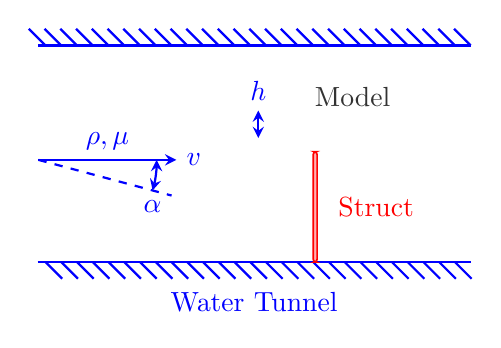
\begin{tikzpicture}[
 interface/.style={
        postaction={draw,decorate,decoration={border,angle=-45,
                    amplitude=0.3cm,segment length=2mm}}}]
\node[blue] at (1.25,-2.5) {Water Tunnel};
\node[black!80] at (2.5,0.1) {Model};
\node[red] at (2.8,-1.3) {Struct};

\draw[thick,interface,blue] (4,0.75)--(-1.5,0.75)  (-1.5,-2)--(4,-2)  ;
\draw[semithick,fill=red!30,draw=red,rounded corners=1](2,-0.6) --(2,-2)--(2.05,-2)--(2.05,-0.6)--cycle;

\begin{scope}[xshift=20,yshift=-5]
% Some profiles look better when using plot[smooth]
 \draw[scale=3, rotate=-15, thick]
            plot file{./figures/airfoil.dat} -- cycle;
\draw[<->,thick,blue,>=stealth] (0.6,-0.25)--(0.6,0.1) node[above] {$h$};
\end{scope}
\begin{scope}[xshift=43,yshift=-20]
\draw [->,thick, blue, >=stealth](-3,0)--(-1.25,0) node[right] {$v$} node[above,midway] {$\rho, \mu$}; 
\draw [thick, blue, >=stealth,dashed](-3,0)--++(-15:1.75);
\draw [<->,thick, blue, >=stealth](-1.5,0) arc(0:-15:1.5) node[below] {$\alpha$};
\end{scope}


\end{tikzpicture}
\caption{\label{fig:2dAircraftModeling}二维翼形的水洞模拟}
\end{minipage}
\end{figure}

表\ref{tab:airfoilINwater}列出了低速小飞机在空气中飞行的参数范围和水洞实验允许的参数值, 以及空气和水的运动粘性系数\cite{fluid_Properties}. 做机翼的模型实验, 考虑到实验时模型的放置方式, 三维模拟时, 尺寸应以翼展方向的缩比为准; 二维模拟时, 尺寸应以翼型厚度方向的缩比为准. \textcolor{blue}{为消除边界影响, 模型的厚度不应大于水洞直径的1/5}.

\begin{table}[!htb]\label{tab:airfoilINwater}
\centering
\caption{水洞做机翼的模型实验与原型的各参量范围}
\begin{tabular}{l|c|c}
\hline 
 & 原型参数实际范围 & 模型参数允许范围\tabularnewline
\hline 
翼展长度$l\,(\mathrm{m})$ & $>8.0$ & $<2.0$\tabularnewline
翼形厚度$h\,(\mathrm{m})$ & $>0.2$ & \textcolor{blue}{$<2/5$}\tabularnewline
\hline 
$v\,(\mathrm{m/s})$ & $>20$ & $<10$\tabularnewline
\hline 
$\nu=\mu/\rho\,(\mathrm{m^{2}/s})$ & $1.5\times 10^{-5}$ & $1.0\times 10^{-6}$\tabularnewline
\hline 
$\mathrm{Re_{3d}} = vl/\nu$ & $>1.0\times 10^7$ & $<2.0\times 10^7$\tabularnewline
$\mathrm{Re_{2d}} = vh/\nu$ & $>1.3\times 10^5$ & $<4\times 10^6$ \tabularnewline
\hline 
\end{tabular}
\end{table}

用表\ref{tab:airfoilINwater}中的参数可分别计算出原型和模型中的几何相似和动力学无量纲相似参数, 几何相似容易满足, 主要考查动力学相似, 通过计算原型和模型中雷诺数的范围(三维和二维模拟情况下的雷诺数范围见表\ref{tab:airfoilINwater}最后两列). \textbf{三维模拟}情况下, 尺寸缩比和速度缩比范围满足以下条件
\[
\alpha_l = \frac{l_\mathrm{p}}{l_\mathrm{m}} > \frac{8}{2}\, , 
\quad 
\alpha_v = \frac{v_\mathrm{p}}{v_\mathrm{m}} > \frac{20}{10}\, , 
\quad 
\alpha_l\cdot \alpha_v = \frac{\nu_\mathrm{p}}{\nu_\mathrm{m}}  = 15
\]
由此可解得尺寸缩比和速度缩比范围分别为
\[
\alpha_l \in (4, 15/2), \qquad \alpha_v \in (2, 15/4)
\]
因此在做三维模拟时, 水洞可以用来模拟翼展长度$l<15\mathrm{m}$, 速度$v<37.5\mathrm{m/s}$的飞机. 若把机翼简化成二维模型, 则可以模拟尺寸更大, 速度更快的飞机. 二维情况下, 尺寸缩比和速度缩比范围满足以下条件
\[
\alpha_l = \frac{h_\mathrm{p}}{h_\mathrm{m}} > \frac{0.2}{2/5}\, , 
\quad 
\alpha_v = \frac{v_\mathrm{p}}{v_\mathrm{m}} >\frac{20}{10}\, , 
\quad 
\alpha_l\cdot \alpha_v = \frac{\nu_\mathrm{p}}{\nu_\mathrm{m}}  = 15
\]
由此可解得尺寸缩比和速度缩比范围分别为
\[
\alpha_l \in (1/2, 15/2), \qquad \alpha_v \in (2, 30)
\]
因此在做\textbf{二维模拟}时, 水洞可以用来模拟翼形高度$h<3\mathrm{m}$, 速度$v<300\mathrm{m/s}$的飞机. 二维模拟能模拟飞机的尺寸和速度比三维模拟的范围更大.

\item \textbf{风洞做潜艇的模型实验:}

\begin{minipage}[c]{0.6\linewidth}

%世界上最大的潜艇是Typhoons\cite{Typhoon}, 长$175\mathrm{m}$, 宽$23\mathrm{m}$, 速度可达$41.15\mathrm{km/h}$.
芬兰海军的Saukko\cite{Saukko}潜艇是世界上最小的潜艇之一, 其长为$32.4\mathrm{m}$, 宽为$4.1\mathrm{m}$, 速度为$10.6\mathrm{km/h}$. 世界上最快的潜艇一般认为是苏联K-222潜艇\cite{K-222}, 速度可达$82.8\mathrm{km/h}$. 低速风洞的直径一般小于$6\mathrm{m}$\cite{baike_wind_tunnel,wike_wind_tunnel}, \textcolor{blue}{为消除边界影响, 模型的宽度不应大于风洞直径的1/3}, \textcolor{red}{这里限制风洞马赫数低于0.3, 即风洞的气流速度低于$100\mathrm{m/s}$}. 
\end{minipage}
\begin{minipage}[c]{0.4\linewidth}
\begin{center}
\usetikzlibrary{%
    decorations.pathreplacing,%
    decorations.pathmorphing,arrows
}

\definecolor{ca5bed6}{RGB}{160,160,160}
\definecolor{c1a232b}{RGB}{30,30,30}
\definecolor{c2c3c57}{RGB}{50,50,50}
\definecolor{c354b6b}{RGB}{80,80,80}
\definecolor{c453f41}{RGB}{70,70,70}
\definecolor{caed0e3}{RGB}{200,200,200}
\definecolor{cffffff}{RGB}{255,255,255}


\definecolor{ceb2f9e}{RGB}{150,150,150}
\definecolor{c231f20}{RGB}{30,30,30}
\definecolor{cf188c6}{RGB}{180,180,180}
\definecolor{cfac2e3}{RGB}{220,220,220}
\definecolor{cec008c}{RGB}{60,60,60}
\definecolor{cf9b2dc}{RGB}{200,200,200}


\begin{tikzpicture}[
 interface/.style={
        postaction={draw,decorate,decoration={border,angle=-45,
                    amplitude=0.3cm,segment length=2mm}}}]
\node[blue] at (1.25,-2.5) {Wind Tunnel};
\node[black!80] at (1.25,0.15) {Model};
\node[red] at (2.5,-1.5) {Struct};

\draw[thick,interface,blue] (4,0.75)--(-1.5,0.75)  (-1.5,-2)--(4,-2)  ;
\draw[semithick,fill=red!30,draw=red,rounded corners=1](2.8,-0.65)--(3.2,-0.65) --(3.2,-2)--(3.15,-2)--(3.15,-0.7)--(2.8,-0.7)--cycle;
\draw [->,thick, blue, >=stealth'](-1.5,-0.6)--(-0.35,-0.6) node[above,midway] {$v$} node[below,midway] {$\mu, \rho$};

\draw[thick,blue](3.25,-0.1)--(3.75,-0.1) (3.25,-1)--(3.75,-1);
\draw[thick,blue,<->,>=stealth'] (3.5,-0.1)--(3.5,-1) node[midway,right] {$l$};

\begin{scope}[y=0.80pt, x=0.8pt,yscale=-1,yshift=-1231,xshift=4,scale=1.5]
  \begin{scope}[cm={{0.125,0.0,0.0,-0.125,(-449.47783,1529.2107)}}]
      \path[ball color = gray!30] (4108.1200,3901.0700) .. controls
        (4108.1200,3880.5400) and (3981.6500,3845.4700) .. (3803.9100,3845.4700) ..
        controls (3664.9500,3845.4700) and (3604.9100,3870.3700) ..
        (3604.9100,3901.0700) .. controls (3604.9100,3931.8000) and
        (3664.9500,3956.7000) .. (3803.9100,3956.7000) .. controls
        (3981.6500,3956.7000) and (4108.1200,3921.9500) .. (4108.1200,3901.0700);
      \path[nonzero rule] (4108.1200,3901.0700) .. controls (4108.1200,3880.5400) and
        (3981.6500,3845.4700) .. (3803.9100,3845.4700) .. controls
        (3664.9500,3845.4700) and (3604.9100,3870.3700) .. (3604.9100,3901.0700) ..
        controls (3604.9100,3931.8000) and (3664.9500,3956.7000) ..
        (3803.9100,3956.7000) .. controls (3981.6500,3956.7000) and
        (4108.1200,3921.9500) .. (4108.1200,3901.0700);
  \end{scope}
  \begin{scope}[cm={{0.125,0.0,0.0,-0.125,(-449.47783,1529.2107)}}]
      \path[draw=c231f20] (4108.1200,3901.0700) .. controls (4108.1200,3880.5400) and
        (3981.6500,3845.4700) .. (3803.9100,3845.4700) .. controls
        (3664.9500,3845.4700) and (3604.9100,3870.3700) .. (3604.9100,3901.0700) ..
        controls (3604.9100,3931.8000) and (3664.9500,3956.7000) ..
        (3803.9100,3956.7000) .. controls (3981.6500,3956.7000) and
        (4108.1200,3921.9500) .. (4108.1200,3901.0700) -- cycle;
  \end{scope}
  \begin{scope}[cm={{0.125,0.0,0.0,-0.125,(-449.47783,1529.2107)}}]
      \path[fill=ceb2f9e] (3916.4700,3951.7500) .. controls
        (3916.4700,3951.7500) and (3875.5400,3948.7200) .. (3851.8000,3948.7200) ..
        controls (3808.8500,3948.7200) and (3808.3500,3956.6100) ..
        (3808.3500,3956.6100) -- (3808.3500,4000.4500) .. controls
        (3808.3500,4002.8400) and (3810.3000,4004.8000) .. (3812.7000,4004.8000) --
        (3895.9600,4004.8000) .. controls (3898.3400,4004.8000) and
        (3900.3100,4002.8400) .. (3900.3100,4000.4500) -- (3916.4700,3951.7500);
      \path (3916.4700,3951.7500) .. controls (3916.4700,3951.7500) and
        (3875.5400,3948.7200) .. (3851.8000,3948.7200) .. controls
        (3808.8500,3948.7200) and (3808.3500,3956.6100) .. (3808.3500,3956.6100) --
        (3808.3500,4000.4500) .. controls (3808.3500,4002.8400) and
        (3810.3000,4004.8000) .. (3812.7000,4004.8000) -- (3895.9600,4004.8000) ..
        controls (3898.3400,4004.8000) and (3900.3100,4002.8400) ..
        (3900.3100,4000.4500) -- (3916.4700,3951.7500);
  \end{scope}
  \begin{scope}[cm={{0.125,0.0,0.0,-0.125,(-449.47783,1529.2107)}}]
      \path[draw=c231f20] (3916.4700,3951.7500) .. controls (3916.4700,3951.7500) and
        (3875.5400,3948.7200) .. (3851.8000,3948.7200) .. controls
        (3808.8500,3948.7200) and (3808.3500,3956.6100) .. (3808.3500,3956.6100) --
        (3808.3500,4000.4500) .. controls (3808.3500,4002.8400) and
        (3810.3000,4004.8000) .. (3812.7000,4004.8000) -- (3895.9600,4004.8000) ..
        controls (3898.3400,4004.8000) and (3900.3100,4002.8400) ..
        (3900.3100,4000.4500) -- (3916.4700,3951.7500) -- cycle;
  \end{scope}
  \begin{scope}[cm={{0.125,0.0,0.0,-0.125,(-449.47783,1529.2107)}}]
      \path[fill=cf188c6] (4099.3700,3910.3200) -- (4087.7400,3977.0100)
        .. controls (4087.7400,3977.0100) and (4073.1100,3977.5100) ..
        (4061.9900,3977.5100) .. controls (4050.8700,3977.5100) and
        (4045.3100,3978.0300) .. (4038.2400,3968.4200) .. controls
        (4031.1700,3958.8300) and (4012.8100,3928.3100) .. (4010.4500,3924.4700) ..
        controls (4002.3600,3911.3300) and (4034.7000,3922.4400) ..
        (4099.3700,3910.3200);
      \path(4099.3700,3910.3200) -- (4087.7400,3977.0100) .. controls
        (4087.7400,3977.0100) and (4073.1100,3977.5100) .. (4061.9900,3977.5100) ..
        controls (4050.8700,3977.5100) and (4045.3100,3978.0300) ..
        (4038.2400,3968.4200) .. controls (4031.1700,3958.8300) and
        (4012.8100,3928.3100) .. (4010.4500,3924.4700) .. controls
        (4002.3600,3911.3300) and (4034.7000,3922.4400) .. (4099.3700,3910.3200);
  \end{scope}
  \begin{scope}[cm={{0.125,0.0,0.0,-0.125,(-449.47783,1529.2107)}}]
      \path[draw=c231f20] (4099.3700,3910.3200) -- (4087.7400,3977.0100) .. controls
        (4087.7400,3977.0100) and (4073.1100,3977.5100) .. (4061.9900,3977.5100) ..
        controls (4050.8700,3977.5100) and (4045.3100,3978.0300) ..
        (4038.2400,3968.4200) .. controls (4031.1700,3958.8300) and
        (4012.8100,3928.3100) .. (4010.4500,3924.4700) .. controls
        (4002.3600,3911.3300) and (4034.7000,3922.4400) .. (4099.3700,3910.3200) --
        cycle;
      \path[fill=cfac2e3] (4086.3200,3975.5000) .. controls
        (4086.3200,3975.5000) and (4061.5900,3976.0400) .. (4056.6900,3976.0400) ..
        controls (4051.8000,3976.0400) and (4047.7200,3975.2300) ..
        (4045.5500,3973.6000) .. controls (4045.5500,3973.6000) and
        (4051.8000,3973.0600) .. (4063.2100,3973.3300) .. controls
        (4074.6300,3973.6000) and (4086.3200,3975.5000) .. (4086.3200,3975.5000);
      \path[fill=cec008c] (4085.5100,3975.2300) .. controls
        (4082.0800,3973.9400) and (4078.1800,3974.3200) .. (4074.6300,3973.6300) ..
        controls (4072.1000,3973.1400) and (4069.6300,3972.8400) ..
        (4067.0200,3972.7900) .. controls (4064.3200,3972.7400) and
        (4061.5400,3972.6300) .. (4058.8500,3972.7900) .. controls
        (4056.6600,3972.9200) and (4053.2500,3972.6000) .. (4051.3500,3973.6200) ..
        controls (4058.4300,3973.7100) and (4065.5400,3973.2900) ..
        (4072.5700,3974.0100) .. controls (4074.9800,3974.2500) and
        (4077.4700,3974.2400) .. (4079.8100,3974.6800) .. controls
        (4081.6600,3975.0400) and (4084.3400,3974.8300) .. (4086.0500,3975.5000);
      \path[fill=cec008c] (4053.9800,3972.7800) .. controls
        (4051.5200,3971.5000) and (4047.5100,3973.6300) .. (4044.8200,3973.3100) ..
        controls (4046.5000,3974.9600) and (4050.3200,3974.0000) ..
        (4052.5700,3973.8700) .. controls (4055.2700,3973.7200) and
        (4057.8100,3973.0500) .. (4060.6400,3973.0600) .. controls
        (4066.0000,3973.0700) and (4071.7700,3972.9600) .. (4077.0700,3973.6600) ..
        controls (4079.5300,3973.9800) and (4083.1300,3975.0800) ..
        (4085.4200,3974.7700) .. controls (4083.8400,3973.1600) and
        (4080.4600,3973.3100) .. (4078.3800,3973.0900) .. controls
        (4075.5000,3972.7900) and (4072.6100,3972.6800) .. (4069.7400,3972.3700) ..
        controls (4066.3400,3972.0100) and (4063.1600,3971.6100) ..
        (4059.7100,3971.6900) .. controls (4055.3300,3971.8000) and
        (4049.8900,3972.2300) .. (4045.8200,3973.8700);
  \end{scope}
  \begin{scope}[cm={{0.125,0.0,0.0,-0.125,(-449.47783,1529.2107)}}]
      \path[fill=cf188c6] (4099.3700,3891.0700) -- (4087.7400,3824.3800)
        .. controls (4087.7400,3824.3800) and (4073.1100,3823.8800) ..
        (4061.9900,3823.8800) .. controls (4050.8700,3823.8800) and
        (4045.3100,3823.3700) .. (4038.2400,3832.9700) .. controls
        (4031.1700,3842.5700) and (4012.8100,3873.0800) .. (4010.4500,3876.9300) ..
        controls (4002.3600,3890.0600) and (4034.7000,3878.9500) ..
        (4099.3700,3891.0700);
      \path[nonzero rule] (4099.3700,3891.0700) -- (4087.7400,3824.3800) .. controls
        (4087.7400,3824.3800) and (4073.1100,3823.8800) .. (4061.9900,3823.8800) ..
        controls (4050.8700,3823.8800) and (4045.3100,3823.3700) ..
        (4038.2400,3832.9700) .. controls (4031.1700,3842.5700) and
        (4012.8100,3873.0800) .. (4010.4500,3876.9300) .. controls
        (4002.3600,3890.0600) and (4034.7000,3878.9500) .. (4099.3700,3891.0700);
  \end{scope}
  \begin{scope}[cm={{0.125,0.0,0.0,-0.125,(-449.47783,1529.2107)}}]
      \path[draw=c231f20] (4099.3700,3891.0700) -- (4087.7400,3824.3800) .. controls
        (4087.7400,3824.3800) and (4073.1100,3823.8800) .. (4061.9900,3823.8800) ..
        controls (4050.8700,3823.8800) and (4045.3100,3823.3700) ..
        (4038.2400,3832.9700) .. controls (4031.1700,3842.5700) and
        (4012.8100,3873.0800) .. (4010.4500,3876.9300) .. controls
        (4002.3600,3890.0600) and (4034.7000,3878.9500) .. (4099.3700,3891.0700) --
        cycle;
      \path[fill=cec008c] (4086.3200,3825.8900) .. controls
        (4086.3200,3825.8900) and (4061.5900,3825.3400) .. (4056.6900,3825.3400) ..
        controls (4051.8000,3825.3400) and (4047.7200,3826.1600) ..
        (4045.5500,3827.8000) .. controls (4045.5500,3827.8000) and
        (4051.8000,3828.3400) .. (4063.2100,3828.0700) .. controls
        (4074.6300,3827.8000) and (4086.3200,3825.8900) .. (4086.3200,3825.8900);
      \path[fill=cec008c] (4085.5100,3826.1600) .. controls
        (4082.0800,3827.4600) and (4078.1800,3827.0700) .. (4074.6300,3827.7600) ..
        controls (4072.1000,3828.2600) and (4069.6300,3828.5500) ..
        (4067.0200,3828.6000) .. controls (4064.3200,3828.6600) and
        (4061.5400,3828.7500) .. (4058.8500,3828.6000) .. controls
        (4056.6600,3828.4800) and (4053.2500,3828.8000) .. (4051.3500,3827.7800) ..
        controls (4058.4300,3827.6800) and (4065.5400,3828.1100) ..
        (4072.5700,3827.3900) .. controls (4074.9800,3827.1400) and
        (4077.4700,3827.1500) .. (4079.8100,3826.7100) .. controls
        (4081.6600,3826.3600) and (4084.3400,3826.5500) .. (4086.0500,3825.8900);
      \path[fill=cec008c] (4053.9800,3828.6100) .. controls
        (4051.5200,3829.8900) and (4047.5100,3827.7700) .. (4044.8200,3828.0900) ..
        controls (4046.5000,3826.4400) and (4050.3200,3827.4000) ..
        (4052.5700,3827.5200) .. controls (4055.2700,3827.6800) and
        (4057.8100,3828.3400) .. (4060.6400,3828.3400) .. controls
        (4066.0000,3828.3300) and (4071.7700,3828.4200) .. (4077.0700,3827.7300) ..
        controls (4079.5300,3827.4100) and (4083.1300,3826.3200) ..
        (4085.4200,3826.6200) .. controls (4083.8400,3828.2300) and
        (4080.4600,3828.0900) .. (4078.3800,3828.3000) .. controls
        (4075.5000,3828.6000) and (4072.6100,3828.7100) .. (4069.7400,3829.0200) ..
        controls (4066.3400,3829.3900) and (4063.1600,3829.7900) ..
        (4059.7100,3829.7000) .. controls (4055.3300,3829.6000) and
        (4049.8900,3829.1600) .. (4045.8200,3827.5200);
  \end{scope}
  \begin{scope}[cm={{0.125,0.0,0.0,-0.125,(-449.47783,1529.2107)}}]
      \path[fill=ceb2f9e] (3990.9200,3884.9500) .. controls
        (3989.4300,3884.7700) and (3841.0800,3866.7100) .. (3721.7900,3881.6900) ..
        controls (3719.4000,3881.9800) and (3717.2300,3880.2900) ..
        (3716.9300,3877.9100) .. controls (3716.6300,3875.5300) and
        (3718.3100,3873.3500) .. (3720.7000,3873.0600) .. controls
        (3841.0800,3857.9400) and (3990.4900,3876.1300) .. (3991.9900,3876.3200) ..
        controls (3994.3700,3876.6100) and (3996.0600,3878.7800) ..
        (3995.7600,3881.1600) .. controls (3995.4800,3883.5500) and
        (3993.3000,3885.2400) .. (3990.9200,3884.9500);
      \path (3990.9200,3884.9500) .. controls (3989.4300,3884.7700) and
        (3841.0800,3866.7100) .. (3721.7900,3881.6900) .. controls
        (3719.4000,3881.9800) and (3717.2300,3880.2900) .. (3716.9300,3877.9100) ..
        controls (3716.6300,3875.5300) and (3718.3100,3873.3500) ..
        (3720.7000,3873.0600) .. controls (3841.0800,3857.9400) and
        (3990.4900,3876.1300) .. (3991.9900,3876.3200) .. controls
        (3994.3700,3876.6100) and (3996.0600,3878.7800) .. (3995.7600,3881.1600) ..
        controls (3995.4800,3883.5500) and (3993.3000,3885.2400) ..
        (3990.9200,3884.9500);
  \end{scope}
  \path[draw=c231f20] (49.3872,1043.5919) .. controls (49.2009,1043.6149) and
    (30.6572,1045.8719) .. (15.7459,1043.9994) .. controls (15.4472,1043.9634) and
    (15.1759,1044.1744) .. (15.1384,1044.4719) .. controls (15.1009,1044.7694) and
    (15.3109,1045.0419) .. (15.6097,1045.0781) .. controls (30.6572,1046.9681) and
    (49.3334,1044.6944) .. (49.5209,1044.6706) .. controls (49.8184,1044.6346) and
    (50.0297,1044.3631) .. (49.9922,1044.0656) .. controls (49.9572,1043.7669) and
    (49.6847,1043.5556) .. (49.3872,1043.5919) -- cycle(59.1034,1043.3156) --
    (59.1034,1039.8506);
  \path[draw=cec008c] (26.9597,1030.6081) -- (38.3759,1030.6081)(52.0359,1038.0831)
    .. controls (52.0359,1038.0831) and (42.4534,1036.7244) .. (25.2597,1036.4519)
    .. controls (8.0659,1036.1806) and (3.4447,1038.6944) .. (3.4447,1038.6944) --
    (3.4447,1044.5394)(3.5809,1039.5094) .. controls (3.5809,1039.5094) and
    (10.5134,1037.8794) .. (19.2784,1037.8794) .. controls (24.3772,1037.8794) and
    (45.0359,1038.1506) .. (51.4922,1038.8306);
  \path[draw=cf9b2dc,line join=miter,line cap=butt,miter limit=4.00,line
    width=0.261pt] (27.0947,1028.9081) -- (37.3334,1028.9081);

\end{scope}



\end{tikzpicture}

\end{center}
\end{minipage}

表\ref{tab:submarineINair}列出了潜艇在水中前进的参数范围和风洞实验允许的参数值.
用类似``水洞做机翼的模型实验''的讨论方法, 对风洞做潜艇的模型实验进行讨论和分析. 通过计算发现原型和模型的雷诺数(见表\ref{tab:submarineINair})范围有交集, 用风洞做小尺寸, 低速度小尺寸潜艇的模型实验是可行的.
\begin{table}[!htb]\label{tab:submarineINair}
\centering
\caption{风洞做潜艇的模型实验与原型的各参量范围}
\begin{tabular}{c|ccc|c}
\hline 
 &潜艇宽度$l$$(\mathrm{m})$ & $v$$(\mathrm{m/s})$ & $\nu=\mu/\rho$$(\mathrm{m^2/s})$ & $\mathrm{Re}=vl/\nu$\tabularnewline
\hline 
原型 & $>4$ & $>2$ & $1.0\times 10^{-6}$ & $>8.0\times 10^6$\tabularnewline
\hline 
模型 & \textcolor{blue}{$<6/3$} & \textcolor{red}{$<100$} & $1.5\times 10^{-5}$ & $<1.3\times 10^7$\tabularnewline
\hline 
\end{tabular}
\end{table}

尺寸和速度的缩比范围满足
\[
\alpha_l>\frac{4}{6/3}, \quad \alpha_v>\frac{2}{100}, \quad \alpha_l\cdot \alpha_v = \frac{\nu_\mathrm{p}}{\nu_\mathrm{m}} = \frac{1}{15}
\]
由此可解得尺寸缩比和速度缩比范围分别为
\[
\alpha_l \in (2,10/3), \quad \alpha_v \in (1/50, 1/30)
\]
因此在做风洞做潜艇的模型实验时, 风洞可以用来模拟宽$l<20/3=6.7\mathrm{m}$, 速度$v<100/30=3.3\mathrm{m/s}$的潜艇.

\end{enumerate}
\end{solution}
\label{problem:12}

\invisiblesubsection{船舶润湿面积}
\begin{problem}[13]
作船舶润湿面积的量纲分析.
\end{problem}
% --------------------------------------------------------------------
\begin{solution}
\begin{minipage}[c]{0.8\linewidth}
船舶润湿面积$S$与船舶特征常度$l$, 排水体积$D$及行进速度$v$, 水的密度$\rho$及粘性系数$\mu$, 重力加速度$g$有关, 则有
\[
S = f(l,D; v; \rho, \mu, g)
\]
\end{minipage}
\begin{minipage}[c]{0.2\linewidth}
\begin{center}
\usetikzlibrary{calc,intersections,through,backgrounds}
\usetikzlibrary{decorations.pathreplacing,decorations.pathmorphing,arrows}
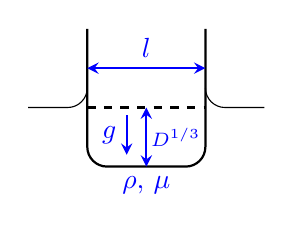
\begin{tikzpicture}
\draw [thick] (-0.75,1)--(-0.75,-0.5) arc(-180:-90:0.25)--(0.5,-0.75) node[below,midway,blue]{$\rho$, $\mu$} arc(-90:0:0.25) -- (0.75,1);
\draw[thick,blue,<->,>=stealth] (-0.75,0.5)--(0.75,0.5) node[above, midway]{$l$};
\draw[thick,dashed] (-0.75,0)--(0.75,0);
\draw (-1.5,0)--(-1,0) arc(-90:0:0.25) (1.5,0)--(1,0) arc(270:180:0.25);
\draw[thick,blue,->,>=stealth] (-0.25,-0.1)--(-0.25,-0.6) node [left,midway]{$g$};
\draw[thick,blue,<->,>=stealth] (0,0)--(0,-0.75) node [right=-2pt,midway,font=\scriptsize]{$D^{1/3}$};
\end{tikzpicture}
\end{center}
\end{minipage}\vspace{5pt}
上式中的各物理量的量纲分别为: $[S]=L^2$, $[l]=L$, $[D]=L^3$, $[v]=LT^{-1}$, $[\rho]=ML^{-3}$, $[\mu]=ML^{-1}T^{-1}$, $[g]=LT^{-2}$. 取$l$, $v$, $\rho$作为基本量, 且作为本问题的单位系统, 用以度量问题中的各量, 于是上式转化为
\[
\frac{S}{l^2} = f\bigg(1,\frac{D}{l^3};1,1,\frac{\mu}{\rho v l}, \frac{g}{v^2/l}\bigg)
\quad\Longrightarrow\quad
S = l^2 f\bigg(\frac{D^{1/3}}{l}, \frac{\rho v l}{\mu}, \frac{gl}{v^2}\bigg) = l^2 f(\Psi, \mathrm{Re}, \mathrm{Fr})
\]
其中无量纲数$\Psi$是几何长度之比, 反映相对载重量; $\mathrm{Re}$为雷诺数; $\mathrm{Fr}$为弗劳德数.
\end{solution}

\invisiblesubsection{轴承问题是否该考虑惯性}
\begin{problem}[14]
轴承问题中是否应该考虑惯性力的作用? 说明理由.
\end{problem}
% --------------------------------------------------------------------
\begin{solution}
\begin{minipage}[c]{0.8\linewidth}
如右图所示, 定承半径为$R$, 滑面平均间隙为$h$(轴的半径$r=R-h$), 润滑介质的粘性系数为$\mu$, 密度为$\rho$, 环境压力为$p_0$, 轴所担负的载重为$W$, 滑面相对速度$v$. 
在轴承润滑问题中, 存在三种力, 即惯性力, 粘性力和压力. 标志惯性力和粘性力之比为
\[
\frac{\text{惯性力}}{\text{粘性力}}=(\mathrm{Re})_h\cdot \frac{h}{R} < 10^{-3} \ll 1
\]
\end{minipage}
\begin{minipage}[c]{0.2\linewidth}
\begin{center}
\usetikzlibrary{calc,intersections,through,backgrounds}
\usetikzlibrary{decorations.pathreplacing,decorations.pathmorphing,arrows}
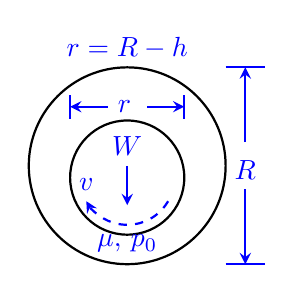
\begin{tikzpicture}
   \draw[thick] (0,0) circle(1.25) (0,-0.15) circle(0.725) node[below=17pt,blue]{$\mu$, $p_0$};
   \draw[thick,blue,->,>=stealth, dashed](0,-0.15)++(-30:0.6) arc(-30:-150:0.6) node[above] {$v$};
  \draw [thick,blue,->,>=stealth](0,0) node[above]{$W$}--(0,-0.5);
  \draw[thick,blue] (1.25,-1.25) -- (1.75,-1.25) (1.25,1.25) -- (1.75,1.25)
                                     (-0.725,0.6)--(-0.725,0.9) (0.725,0.6)--(0.725,0.9);

  \draw[thick,blue,<-,>=stealth] (1.5,-1.25)--(1.5,-0.3) node[above]{$R$};
  \draw[thick,blue,->,>=stealth](1.5,0.3)--(1.5,1.25);
 \node[blue] at (0,1.5){$r=R-h$};

  \draw[thick,blue,<-,>=stealth] (-0.725,0.75)--(-0.25,0.75) node[right]{$r$};
  \draw[thick,blue,<-,>=stealth] (0.725,0.75)--(0.25,0.75);
\end{tikzpicture}
\end{center}
\end{minipage}\vspace{5pt}
其中$(\mathrm{Re})_h=\rho v h/\mu$. 所以可忽略惯性力的影响.
\end{solution}

\invisiblesubsection{小球在粘流中的最终速度和粘性阻力}
\begin{problem}[15]
分析小球在粘性流体中下落的最终速度和粘性阻力(把结果与Stokes公式做对比).
\end{problem}
% --------------------------------------------------------------------
\begin{solution}
\begin{minipage}[c]{0.8\linewidth}
\textbf{最终速度:} 小球在粘性流体中下落的最终速度$v$, 与小球的直径$d$和密度$\rho_\mathrm{s}$, 流体的密度$\rho$和粘性系数$\mu$, 以及重力加速度$g$有关. 显然对于小球的最终速度, 小球的密度$\rho_\mathrm{s}$和流体的密度$\rho$是以差的形式出现的, 因此有
\[
v = f(\rho_\mathrm{s}-\rho, d, \mu, g)
\]
上式中各物理量的量纲分别为: $[v]=LT^{-1}$, $[\rho_\mathrm{s}-\rho]=ML^{-3}$, $[d]=L$, $\mu=ML^{-1}T^{-1}$, $[g]=LT^{-2}$. 以$\rho_\mathrm{s}-\rho$, $\mu$和$d$为基本量, 并作为本问题的单位系统, 来度量问题中的各量, 于是上式转化为
\end{minipage}
\begin{minipage}[c]{0.2\linewidth}
\begin{center}
\usetikzlibrary{calc,intersections,through,backgrounds}
\usetikzlibrary{decorations.pathreplacing,decorations.pathmorphing,arrows}
\usetikzlibrary{shadows}
\begin{tikzpicture}


\node at (0,0) {\includegraphics[width=75pt]{./figures/Stokes_sphere.pdf}};
\shadedraw [ball color= gray!30,thick] (0,0) circle (0.3);
\draw[blue,thick](0.6,0.3) -- (0.9,0.3) (0.6,-0.3) -- (0.9,-0.3);
\draw[blue,thick,<->,>=stealth](0.75,0.3) -- (0.75,-0.3) node[right, midway] {$d$};
\node[blue] at (0,0) {$\rho_\mathrm{s}$};
\draw[blue,->, >=stealth, thick](-0.75,-0.3) -- (-0.75,-1) node[below]{$g$};
\draw[blue] (-0.75,0.5) node{$\rho$, $\mu$};
\draw[blue,->, >=stealth, thick] (0,-0.3)--(0,-1) node[below] {$G$};
\draw[blue,->, >=stealth, thick] (0,0.3)--(0,1) node[above] {$F_\mathrm{b}+F_\mathrm{v}$};

\end{tikzpicture}

\end{center}
\end{minipage}\vspace{5pt}
\[
\frac{v}{\mu/[(\rho_s-\rho)d]} = f\bigg(1,1,1,\frac{g}{\mu^2/[(\rho_s-\rho)^2 d^3]}\bigg) 
\quad\Longrightarrow\quad
v = \frac{\mu}{(\rho_s-\rho)d}f\bigg(\frac{g(\rho_s-\rho)^2d^3}{\mu^2}\bigg)
\]
从\textcolor{blue}{粘性阻力}(见下文式\ref{eq:15Fv-eq-cuvd})的分析中可知, 最终小球所受粘性阻力$F=C\mu v d$为常数, 即$\mu$与$v$成反比, 因此上式可化简为
\[
v = C\cdot\frac{\mu}{(\rho_s-\rho)d} \cdot \frac{g(\rho_s-\rho)^2d^3}{\mu^2} 
= C\cdot\frac{\rho_s-\rho}{\mu} d^2 g
\]
其中$C$为常数, 对比由Stokes公式得到的结果: $v = \frac{(\rho_s-\rho)gd^2}{18\mu}$, 可知上式中$C$的值为$C = 1/18$.

\vspace{10pt}

\noindent\textbf{粘性阻力:} 小球在粘性流体中下落平衡后速度为定值$v$. 粘性阻力$F_\mathrm{v}$最终将恒定, 与小球直径$d$, 流体的密度$\rho$和粘性系数$\mu$, 及最终下落速度$v$有关:
\[
F_\mathrm{v} = f(\rho, \mu, v, d)
\]
其中$F_\mathrm{v}$的量纲为$[F_\mathrm{v}]=MLT^{-2}$. 选取$\mu$, $v$和$d$为基本量, 并作为本问题的单位系统, 来度量问题中的各量, 于是上式转化为
\begin{equation}\label{eq:15Fv-eq-cuvd}
\frac{F_\mathrm{v}}{\mu vd} = f\bigg(\frac{\rho v d}{\mu},1,1,1\bigg)
\quad\Longrightarrow\quad
F_\mathrm{v} = f(\mathrm{Re}) \mu vd
\end{equation}
该问题的雷诺数$\mathrm{Re}\ll 1$, 因此$f(\mathrm{Re})=C$为常数. 对比由Stokes公式得到的结果: $F_\mathrm{v} = 3\pi \mu vd$, 可知常数$C=3\pi$.
\vspace{10pt}

\noindent\textcolor{blue}{从另一角度, 也可求得粘性阻力}. 小球在粘性流体中下落平衡后速度为定值, 则所受重力$G$和浮力$F_b$, 粘性阻力$F_v$平衡, 即 
\begin{equation}\label{eq:15Fv-eq-G-Fb}
F_v = G - F_b = \rho_s V g - \rho V g = \frac{1}{6}\pi (\rho_s - \rho) d^3 g
\end{equation}
进一步由式(\ref{eq:15Fv-eq-cuvd})和式(\ref{eq:15Fv-eq-G-Fb})也可求得小球在粘性流体中下落的最终速度
\[
v = \frac{1}{18}\frac{\rho_s-\rho}{\mu} d^2 g, \qquad
\mu = \frac{1}{18}\frac{\rho_s-\rho}{v}d^2 g
\]
利用上右式可用来测定未知流体的粘性系数.
\end{solution}

\invisiblesubsection{表面张力对水波波速的影响}
\begin{problem}[16]
什么条件下可以不考虑表面张力对水波波速的影响, 从物理上作简单分析.
\end{problem}
% --------------------------------------------------------------------
\begin{solution}
水波在水面传播的过程主要由于惯性和恢复力共同作用引起的. 恢复力主要是重力和水的表面张力(波长较长时忽略), \textbf{定性分析}:

\vspace{5pt}

\noindent
\begin{minipage}[c]{0.7\linewidth}
\begin{itemize} 
\item 当波长$\lambda$较长, 使水面恢复平面形状的恢复力主要是重力, 相比于重力和惯性, 表面张力微不足道, 可以不考虑. 
\item 当波长$\lambda$较短, 水的表面张力也是一种使水面恢复平面形状的有效恢复力, 此时必需考虑表面张力.
\end{itemize}
\end{minipage}
\begin{minipage}[c]{0.3\linewidth}
\begin{center}
\usetikzlibrary{calc,intersections,through,backgrounds}
\usetikzlibrary{decorations.pathreplacing,decorations.pathmorphing,arrows}
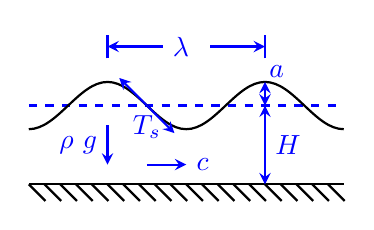
\begin{tikzpicture}[ media/.style={font={\footnotesize\sffamily}},
    interface/.style={
        postaction={draw,decorate,decoration={border,angle=-45,
                    amplitude=0.3cm,segment length=2mm}}}]
\draw[thick,interface] (-2,0)--(2,0);
\draw[thick,dashed,blue](-2,1)--(2,1);
%\draw[thick] (-2,0.75) arc (-90:-15:0.5 and 0.25); %arc(180:0:0.5 and 0.25);
\draw[thick] (-2,0.7) cos (-1.5,1) sin(-1,1.3) cos(-0.5,1) sin(0,0.7) cos(0.5,1) sin(1,1.3) cos(1.5,1) sin(2,0.7);
\draw [thick,blue] (-1,1.6) -- (-1,1.9) (1,1.6) -- (1,1.9);
\draw [thick,blue,<-,>=stealth] (-1,1.75) -- (-0.3,1.75) node[right]{$\lambda$};
\draw [thick,blue,<-,>=stealth] (1,1.75) -- (0.3,1.75);
\draw [thick,blue,<->,>=stealth] (-0.15,0.65)--(-0.85,1.35) node[below,midway]{$T_s$};
\draw [thick,blue,<->,>=stealth] (1,0)--(1,1) node[right,midway]{$H$};
\draw [thick,blue,<->,>=stealth] (1,1)--(1,1.3) node[above right=-3pt]{$a$};
\draw [thick,blue,->,>=stealth] (-0.5,0.25)--(0,0.25) node[right] {$c$};
\draw [thick,blue,->,>=stealth] (-1,0.75)--(-1,0.25) node[midway,left] {$\rho$ $g$};
\end{tikzpicture}
\end{center}
\end{minipage}\vspace{10pt}

\noindent
下面分别从量纲分析角度和水波理论角度进行讨论:
\begin{itemize}
\item \textbf{量纲分析:}
水波波速$c$与水的密度$\rho$, 表面张力$T_s$, 重力加速度$g$, 水波波长$\lambda$, 波幅$a$, 水深$H$有关:
\[
c = f(\rho,g,\lambda,a,H,T_s)
\]
上式中各物理量的量纲分别为: $[c]=LT^{-1}$, $\rho=ML^{-3}$, $[g]=LT^{-2}$, $[\lambda]=[a]=[H]=L$, $[T_s]=MT^{-2}$. 选取$\rho$, $g$, $H$作基本量, 并作为本问题的单位系统, 用以度量问题中的各量, 于是, 上式转化为
\[
\frac{c}{\sqrt{gH}} = f\bigg(1,1,\frac{\lambda}{H}, \frac{a}{H}, 1, \frac{T_s}{\rho g H^2}\bigg) = f\bigg(\frac{\lambda}{H},\frac{a}{H},\frac{T_s}{\rho g \lambda^2}\cdot\Big(\frac{\lambda}{H}\Big)^2\bigg) = f\bigg(\frac{\lambda}{H}, \frac{a}{H}, \frac{T_s}{\rho g \lambda^2}\bigg)
\]
观察上式不难发现: 当$\lambda\gg \sqrt{T_s/(\rho g)}$, 即波长$\lambda$较大时, 表面张力对水波波速的影响可以不考虑.

\item \textbf{水波理论:}
水波理论给出$f$的形式是
\[
\frac{c}{\sqrt{gH}} = \bigg[1+\frac{(2\pi)^2T_s}{\rho g \lambda^2}\bigg]^{1/2}\bigg[\frac{2\pi H/\lambda}{2\pi H/\lambda}\bigg]^{1/2}
\]
从上式中的右端第一个因子也可以看出, 当$\frac{(2\pi)^2T_s}{\rho g \lambda^2}\ll 1$即$2\pi\sqrt{T_s/(\rho g)}\ll \lambda$时, 表面张力对水波波速的影响可以不考虑.
\end{itemize}
综上所述, 无论是从定性分析, 还是量纲分析及水波理论, 都可以得出: \textbf{当水波波长较长时, 可以不考虑表面张力对水波波速的影响}.
\end{solution}

\invisiblesubsection{两端固定的梁的挠度}
\begin{problem}[17]
讨论两端固定的梁在分布载荷作用下的挠度.
\end{problem}
% --------------------------------------------------------------------
\begin{solution}
\begin{minipage}[c]{0.7\linewidth}
该问题的控制参数有: 梁的长度$l$, 梁的抗弯刚度$EI$($E$为杨氏模量, $I$为截面矩), 分布载荷$q(x)$(由特征分布载荷$q_m$和表示分布特征的长度$l_q$来表征), 于是挠度应该是坐标$x$和上述参数的函数:
\[
w = f(x; l; EI; q_m, l_q)
\]
\end{minipage}
\begin{minipage}[c]{0.3\linewidth}
\begin{center}
\usetikzlibrary{calc,intersections,through,backgrounds}
\usetikzlibrary{decorations.pathreplacing,decorations.pathmorphing,arrows}
\usetikzlibrary{shapes}
\begin{tikzpicture}
\draw [thick] (-2,-0.5) rectangle (2,0.5);
\draw [thick,blue] (2,0.5) arc (0:180:2 and 0.6) node[midway,above=13pt]{$q$};
\draw[thick,blue,->,>=stealth'] (0.4,1.1)--(0.4,0.5);
\draw[thick,blue,->,>=stealth'] (-0.4,1.1)--(-0.4,0.5);
\draw[thick,blue,->,>=stealth'] (0.8,1.05)--(0.8,0.5);
\draw[thick,blue,->,>=stealth'] (-0.8,1.05)--(-0.8,0.5);
\draw[thick,blue,->,>=stealth'] (1.2,0.98)--(1.2,0.5);
\draw[thick,blue,->,>=stealth'] (-1.2,0.98)--(-1.2,0.5);
\draw[thick,blue,->,>=stealth'] (1.6,0.85)--(1.6,0.5);
\draw[thick,blue,->,>=stealth'] (-1.6,0.85)--(-1.6,0.5);

\draw [thick,blue,dashed] (-2,0.5) arc (210:330:2.3 and 0.75)
                                                    (-2,-0.5) arc (210:330:2.3 and 0.75);
\draw[thick,blue,<->,>=stealth'] (0,-0.5)--(0,-0.89) node[midway,right]{$w$};

\draw (-2,-0.5) node[below,draw=blue,thick,regular polygon, regular polygon sides=3,  inner sep=1.25]{};
\draw (2,-0.5) node[draw=blue,thick,below,regular polygon, regular polygon sides=3,  inner sep=1.25]{};
\draw[thick,blue,>=stealth'](-2,-0.75)--(-2,-1.25) (2,-0.75)--(2,-1.25); \draw[thick,blue,<-,>=stealth'](-2,-1.15)--(-0.25,-1.15) node[right]{$l$}; \draw[thick,blue,<-,>=stealth'](2,-1.15)--(0.25,-1.15);
\end{tikzpicture}
\end{center}
\end{minipage}\vspace{10pt}
上式中的各物理量的量纲分别为:$[w]=[x]=[l]=[l_q]=L$, $[EI]=FL^2$, $[q_m]=FL^{-1}$. 该问题中含有两个独立量纲, 取$l$和$EI$作为基本量, 且组成单位系统, 于是上式可转化为
\begin{equation}\label{eq:17-wl}
\frac{w}{l} = f\bigg(\frac{x}{l},1,1,\frac{q_m}{EI/l^3},\frac{l_q}{l}\bigg)
= f\bigg(\frac{x}{l},\frac{q_ml^3}{EI},\frac{l_q}{l}\bigg)
\end{equation}
因此, 只要保持
\[
\frac{q_ml^3}{EI}=\mathrm{const},\qquad \frac{l_q}{l}=\mathrm{const}
\]
就会有同一个无量纲挠度分布$w = lf(x/l)$. 对比式(\ref{eq:17-wl})与书本\cite{tan_dimensional_2011}第50页式(4.3)的简支梁的结果, 发现结果在形式上一样的, 但由于这两种情形在物理上并不一样, 可知量纲分析的结果中的$f$函数的形式必然不同.
\end{solution}
\label{problem:17}

\invisiblesubsection{悬臂梁的最大挠度与梁长的关系}
\begin{problem}[18]
讨论悬臂梁在自重作用下的最大挠度与梁长的关系.
\end{problem}
% --------------------------------------------------------------------
\begin{solution}
\begin{minipage}[c]{0.7\linewidth}
该问题的控制参数有: 梁的长度$l$, 梁的抗弯刚度$EI$($E$为杨氏模量, $I$为截面矩), 单位长度梁重$q$, 于是最大挠度应该是上述参数的函数:
\[
w_{\max} = f(l; EI; q)
\]
\end{minipage}
\begin{minipage}[c]{0.3\linewidth}
\begin{center}
\usetikzlibrary{calc,intersections,through,backgrounds}
\usetikzlibrary{decorations.pathreplacing,decorations.pathmorphing,arrows}
\usetikzlibrary{shapes}
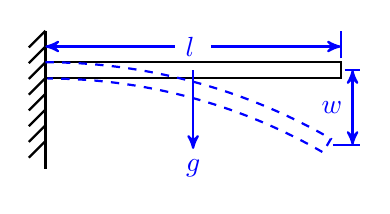
\begin{tikzpicture}[interface/.style={
        postaction={draw,decorate,decoration={border,angle=-45,
                    amplitude=0.3cm,segment length=2mm}}}]
\draw[interface,thick] (0,0.5)--(0,-1.25);
\draw [thick] (0,-0.1) rectangle (3.75,0.1);
\draw [thick,blue,dashed] (0,0.1) arc (90:60:7.25 and 7.25) --++(-0.1,-0.17321)  arc (60:90:7 and 7) ;
\draw [thick,blue,->,>=stealth'](1.875,0)--(1.875,-1) node[below]{$g$};

\draw[thick,blue,<->,>=stealth'] (3.65,-0.95)--(4,-0.95) (3.8,0)--(4,0) (3.9,0)--(3.9,-0.95) node[midway,left]{$w$};

\draw[blue,thick,<-,>=stealth'](3.75,0.15) -- (3.75,0.5) (0,0.3)--(1.65,0.3) node [right]{$l$};
\draw[blue,thick,->,>=stealth'](2.1,0.3)--(3.75,0.3);
\end{tikzpicture}
\end{center}
\end{minipage}\vspace{10pt}

上式中各物理量的量纲分别为: $[w_{\max}]=[l]=L$, $[EI]=FL^2$, $q=FL^{-1}$. 该问题中含两个独立量纲, 取$l$和$EI$作为基本量, 且组成单位系统, 于是上式可转化为
\[
\frac{w_{\max}}{l} = f\bigg(1,1,\frac{q}{EI/l^3}\bigg) 
\quad\Longrightarrow\quad
w = l f\bigg(\frac{ql^3}{EI}\bigg) 
\]
考虑到在弹性范围内有$w_{\max}\propto 1/E$, 与上式对比可得
\[
w_{\max} = C\frac{q}{EI} l^4
\]
其中$C$为常数, 可见悬臂梁在自重作用下的最大挠度$w_{\max}$与梁长的四次方$l^4$成正比.
\end{solution}

\invisiblesubsection{方形空心简支梁的挠度}
\begin{problem}[19]
计论方形空心简支梁的挠度分布, 若用实心梁来模拟, 要求符合什么条件?
\end{problem}
% --------------------------------------------------------------------
\begin{solution}
\begin{minipage}[c]{0.7\linewidth}
由\hyperref[problem:17]{17}题式(\ref{eq:17-wl})结论, 可知若用实心梁来模拟方形空心简支梁的挠度分布, 不必要求模型的截面形状遵守几何相似的条件, 只要求截面矩满足
\end{minipage}
\begin{minipage}[c]{0.3\linewidth}
\begin{center}
\usetikzlibrary{calc,intersections,through,backgrounds}
\usetikzlibrary{decorations.pathreplacing,decorations.pathmorphing,arrows}
\usetikzlibrary{shapes}
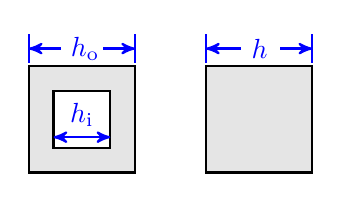
\begin{tikzpicture}[scale=0.9]
\draw[thick,fill=gray!20] (-0.75,-0.75) rectangle(0.75,0.75);
\draw[thick,fill=white]  (-0.4,-0.4) rectangle (0.4,0.4);


\draw[thick,blue,<-,>=stealth'] (-0.75,0.8)--(-0.75,1.2) (0.75,0.8)--(0.75,1.2) (-0.75,1)--(-0.3,1) node[right]{$h_\mathrm{o}$};
\draw[thick,blue,->,>=stealth'] (0.3,1)--(0.75,1) ;
\draw[thick,blue,<->,>=stealth'] (-0.4,-0.25)--(0.4,-0.25) node[midway,above]{$h_\mathrm{i}$} ;


\draw[thick,fill=gray!20] (1.75,-0.75) rectangle(3.25,0.75);
\draw[thick,blue,<-,>=stealth'] (1.75,0.8)--(1.75,1.2) (3.25,0.8)--(3.25,1.2) (1.75,1)--(2.25,1) node[right]{$h$};
\draw[thick,blue,->,>=stealth'] (2.8,1)--(3.25,1) ;
\end{tikzpicture}
\end{center}
\end{minipage}
\[
\bigg(\frac{q_ml^3}{EI}\bigg)_\mathrm{m} = \bigg(\frac{q_ml^3}{EI}\bigg)_\mathrm{p}
\]
对于方形实心简支梁和方形空心简支梁, 截面矩分别为:
\begin{itemize}
\item \textbf{方形实心简支梁}: 边长为$h$, 则$I_\mathrm{m} = h^4/12$.
\item \textbf{方形空心简支梁}: 内外边长分别为$h_\mathrm{i}$, $h_\mathrm{o}$, 则$I_\mathrm{p}=(h_\mathrm{o}^4-h_\mathrm{i}^4)/12$.
\end{itemize}
因此若用实心梁来模拟方形空心简支梁的挠度分布需满足
\[
\Bigg[\frac{q_ml^3}{Eh^4}\Bigg]_\mathrm{m} = \Bigg[\frac{q_ml^3}{E\big(h_\mathrm{o}^4-h_\mathrm{i}^4\big)}\Bigg]_\mathrm{p}
\]
\end{solution}
\label{problem:19}

\invisiblesubsection{需要考虑重力的结构物}
\begin{problem}[20]
什么样的结构物需要考虑重力的作用?
\end{problem}
% --------------------------------------------------------------------
\begin{solution}
设结构物的高度为$h$, 密度为$\rho$, 临界屈服应力$p_\mathrm{cr}$, 重力加速度为$g$, 特征分布载荷为$\Sigma$. 重力所引起的应力大约和$\rho g h$差不多大, 以下情况需要考虑重力的作用:
\begin{itemize}
\item 重力占主导作用或相对于外载并不是很小时, 则显然要考虑重力.
\[
\frac{\rho g h}{\Sigma}\gtrsim 1
\]
如分析悬臂梁在自重作用下的挠度分布(这种情况外载为零).
\item 当结构物的高度$h$较大时, 以至于重力作用超过临界屈服应力或与临界屈服应力相当时, 也需要考虑重力的作用.
\[
\frac{\rho g h}{p_\mathrm{cr}}\gtrsim 1
\]
\end{itemize}
\end{solution}

\invisiblesubsection{国内离心机调查}
\begin{problem}[21]
调查一下国内做结构物的重力效应实验的离心机有多大, 写出主要参数.
\end{problem}
% --------------------------------------------------------------------

\vspace{10pt}
早在上世纪50年代, 我国在前苏联学术界的影响下开始对离心机的应用有所认识. 到60年代后期, 为研究核能和航空航天技术, 有关部门设计制造了几台大尺寸离心机, 但都为训练飞行人员和检验设备使用. 80年代后各大科研单位和高校开始设计和研制离心模型试验设备, 并应用于解决工程问题\cite{centrifugesParameters}. 经过半个世纪的发展, 应用离心机模拟实验技术在我国已得到广泛应用.

\vspace{-14pt}
\noindent\begin{minipage}[b]{0.55\linewidth}
\indent 如右图所示, 离心机的主要参数为: 有效半径$R$, 最大加速度$g_{\max}$, 最大荷载$m_{\max}$, 模型规模, 容量(单位$gt$, $g$为重力加速度, $t$为质量单位:吨). 表\ref{teb:centrifuges}(见第\pageref{teb:centrifuges}页)列出了截止2011年我国主要离心机及主要参数.
\end{minipage}
\begin{minipage}[b]{0.45\linewidth}
\begin{center}
\usetikzlibrary{%
    decorations.pathreplacing,%
    decorations.pathmorphing,arrows
}


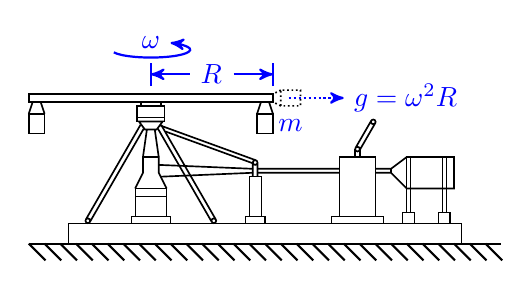
\begin{tikzpicture}[
 interface/.style={
        postaction={draw,decorate,decoration={border,angle=-45,
                    amplitude=0.3cm,segment length=2mm}}}]

\draw[thick,interface] (0,0)--(6,0) ;
\draw (0.5,0.0) rectangle (5.5,0.25)
                                   (1.3,0.25) rectangle (1.8,0.35)
                                   (1.35,0.35) rectangle (1.75,0.6)
                                   (1.35,0.6) rectangle (1.75,0.7)
                                   (2.75,0.25) rectangle (3,0.35)
                                   (2.8,0.35) rectangle (2.95,0.85);

\draw (3.85,0.25) rectangle (4.5,0.35)
             (3.95,0.35) rectangle (4.4,1.1)
             (4.75,0.25) rectangle (4.9,0.4)
             (5.2,0.25) rectangle (5.35,0.4)
             (4.8,0.4) rectangle (4.85,1.1)
             (5.25,0.4) rectangle (5.3,1.1);

\draw[semithick] (4.175,1.2) circle (0.03)
                                  (4.175,1.2) ++(150:0.03)-- ++(60:0.4)
                                  (4.175,1.2) ++(-30:0.03)-- ++(60:0.4)
                                  ++(150:0.03) circle (0.03);
\draw [semithick] (4.145,1.2)--(4.145,1.1)  (4.205,1.2)--(4.205,1.1);

\draw [semithick] (1.65, 1)--(2.85,0.95) (2.85,0.9)--(1.675,0.85)
                                    (2.91,0.95)--(3.95,0.95) (2.91,0.9)--(3.95,0.9)
                                     (4.4,0.95)--(4.6,0.95) (4.4,0.9)--(4.6,0.9)
                                      (4.6,0.9)--(4.6,0.95)--(4.8,1.1)--(5.3,1.1)--(5.4,1.1)--(5.4,0.7)--(4.8,0.7)--cycle;

\draw [semithick] (2.875,1.03)circle(0.03)
                                   (2.845,0.85) --(2.845,1.03) (2.905,0.85)--(2.905,1.03);
\draw [semithick] (2.875,1.03)++(-160:0.03)--++(160:1.18)
                                   (2.875,1.03)++(70:0.03)--++(160:1.3);

\draw[semithick] (1.35,0.7)--(1.45,0.9)--(1.45,1.1)--(1.65,1.1)--(1.65,0.9)--(1.75,0.7)
(1.45,1.1)--(1.5,1.45)--(1.6,1.45)--(1.65,1.1)
(1.5,1.45)--(1.475,1.45)--(1.4,1.55)--(1.7,1.55)--(1.625,1.45)--(1.6,1.45);

\draw[semithick] (1.375,1.55) rectangle (1.725,1.6)
 (1.375,1.6) rectangle (1.725,1.75)
 (1.425,1.75) rectangle (1.675,1.8)
(0,1.8) rectangle(3.1,1.9)
(0,1.4)rectangle (0.2,1.65) 
(2.9,1.4)rectangle (3.1,1.65);
\draw [semithick] (0,1.65)--(0.05,1.8) (0.2,1.65)--(0.15,1.8)
                                    (2.9,1.65)--(2.95,1.8) (3.1,1.65)--(3.05,1.8);
\draw [semithick,densely dotted] (3.2,1.75) rectangle (3.45,1.95) (3.2,1.75)--(3.1,1.8) (3.2,1.95)--(3.1,1.9);

\draw[thick,blue] (1.55,2)--(1.55,2.3) (3.1,2)--(3.1,2.3);
\draw[thick,blue,->,>=stealth'] (2.6,2.15)--(3.1,2.15);
\draw[thick,blue,<-,>=stealth'] (1.55,2.15)--(2.05,2.15) node[right]{$R$};
\draw[blue, thick,->,>=stealth'] (1.55,2.6)++(-160:0.5) arc (-160:60:0.5 and 0.1) node[left]{$\omega$};
\node[blue] at (3.325,1.5) {$m$};
\draw[thick,blue,->,>=stealth',densely dotted] (3.3,1.85)--(4,1.85) node[right]{$g = \omega^2 R$};


\draw[semithick] (0.75,0.29) circle (0.03)
                                  (0.75,0.29) ++(150:0.03)-- ++(60:1.39)
                                  (0.75,0.29) ++(-30:0.03)-- ++(60:1.37);

\draw[semithick] (2.35,0.29) circle (0.03)
                                  (2.35,0.29) ++(210:0.03)-- ++(120:1.37)
                                  (2.35,0.29) ++(30:0.03)-- ++(120:1.39);
\end{tikzpicture}

\end{center}
\end{minipage}


\begin{landscape}
\begin{solution}
\begin{table}[!htb]
\centering
\caption{\label{teb:centrifuges}我国主要离心机及主要技术性能指标\cite{centrifugesParameters}}
{\footnotesize\begin{tabular}{ c c c c c c c c }
\hline 
单位 & 建成时间 & 有效半径/m & 最大加速度/g & 模型规模 & 最大荷载/kg  & 容量/gt & 备注 \tabularnewline
\hline 
中航511厂      & 1960 &6.5 & 80 & 动力 145kW.D.C& 800 & 140 & 飞机工业\tabularnewline
第七机械工业部 &      & 1.7 & 80 & 动力 5kW & 20 &  & 飞机工业\tabularnewline
第二机械工业部 & 1969 & 10.8& 70 & 直径$\times$高度 $0.98 \times 0.88\mathrm{m}$ & 2000 &  & 飞机工业及模拟飞行器\tabularnewline
\hline 
中国工程物理研究院 &  &  &  & 长$\times$宽$\times$高 &  &  & \tabularnewline
第四研究所&1968& 10.8&90 &$0.92\times 0.30\times 0.67 \mathrm{m}$ & 2400 & 216 & 飞机工业及模拟飞行器\tabularnewline
          &1985& 10.8&110&$0.92\times 0.67\times 0.30\mathrm{m}$&3000 & 330 & 主要为军品需求\tabularnewline
\hline 
国防科工委507所&  &  10& 25 &  & 5000 &125 & 模拟飞行器\tabularnewline
华东水利学院(河海大学)&  &2.4&   & $0.48\times 0.28\times 0.15\mathrm{m}$ & 100 & 10 & \tabularnewline
\hline 
                  &1982&2.4&250&$0.90\times0.16\times0.35\mathrm{m}$&100 & 25& \tabularnewline
                  &1982&2.5&300&$0.50\times0.30\times0.15\mathrm{m}$&100 & 20& \tabularnewline
南京水利科学研究院 &    &   &   &$0.45\times0.20\times0.30\mathrm{m}$&    & 30& \tabularnewline
                  &1988&2.1&250&$0.52\times0.40\times0.60\mathrm{m}$&200 & 50& NH-89型\tabularnewline
                  &1992&5.0&200&$1.10\times1.10\times1.10\mathrm{m}$&2000&400& NS-400g\tabularnewline

\hline 
长江水利水电科学院 &1983& 3 &300  &$1.10\times0.33\times0.50\mathrm{m}$&500& 150&\tabularnewline
(长江科学院)       &1983& 3 &300  &$1.10\times0.21\times0.50\mathrm{m}$&10000& 180&\tabularnewline
                  &1985& 3 &300  &$0.76\times0.30\times0.41\mathrm{m}$&1000& 300&\tabularnewline
\hline 
成都勘测设计院 &  & 5 & 200   &  & 1000 & 200 & \tabularnewline
上海铁道学院  &1987&1.55&200 &$0.48\times0.24\times0.32\mathrm{m}$&100&20&L-30型 \tabularnewline
四川(联合)大学  &1990&1.5&250&$0.48\times0.31\times0.30\mathrm{m}$&100&25& \tabularnewline
成都科技大学(今四川大学) &1991&1.54&250 &$0.60\times0.40\times0.40\mathrm{m}$& &25& \tabularnewline
中国水利水电科学研究院  &1993 &4& 300 &$1.50\times1.00\times1.50\mathrm{m}$& & 450&LXJ-4-450 \tabularnewline
  &  &   &    & & &50 & NS-89型\tabularnewline
清华大学  &1993& 2&200&$0.75\times0.50\times0.60\mathrm{m}$&250&50&TH-50gt, 拟静力\tabularnewline
          &  &   &    &$0.50\times0.20\times0.30\mathrm{m}$& &  &动力固壁式\tabularnewline
          &  &   &    &$0.50\times 0.20\times 0.35\mathrm{m}$& &  & 动力叠环式\tabularnewline

香港科技大学&1997&4.5 & 150&$ 1.50\times1.50\times1.60\mathrm{m}$&2670 & 400 &拟静力 \tabularnewline
           &    &    &  75&$ 0.60\times0.60 \times0.4 \mathrm{m}$& &  & 动力\tabularnewline
西南交通大学&2002&2.7&200&$0.60\times 0.40\times0.40\mathrm{m}$&500&100& \tabularnewline
重庆交通大学&2005& 2 &200&$0.70\times0.60\times0.40\mathrm{m}$&300&60& \tabularnewline
长安大学    &2005& 2 &200&$0.60\times0.36\times0.50\mathrm{m}$&300&60& \tabularnewline
同济大学    &2005& 3 &200&$0.70\times0.70\times0.90\mathrm{m}$&750&150&安装机械手\tabularnewline
\hline 

\end{tabular}}
\end{table}
\textcolor{red}{谈老师批注: ``第二机械工业部''和``中国工程物理研究院''为同一单位.} 经本人核实\cite{caep}, 确实如此.
\end{solution}
\end{landscape}

\invisiblesubsection{有限弹性体的固有周期}
\begin{problem}[22]
求有限弹性体的固有周期.
\end{problem}
% --------------------------------------------------------------------
\begin{solution}
有限弹性体的振动实际上是动势能的相互转化现象, 动能源于运动惯性, 由介质的密度$\rho$表征, 弹性势能源于
介质所具有的恢复变形的特性, 由杨氏模量$E$和泊松比$\nu$表征, 因此特征长度为$l,l',l'',\cdots$的有限弹性体的固有周期
\[
\Gamma = f(l,l',l'',\cdots,\rho,E,\nu)
\]
上式中各物理量的量纲分别为: $[\Gamma]=T$, $[l]=[l']=[l'']=\cdots = L$, $[\rho]=ML^{-3}$, $[E]=ML^{-1}T^{-2}$, $\nu$为无量纲常数. 取$l$, $\rho$和$E$作为基本量, 由上式可导出以下无量纲关系:
\[
\frac{\Gamma}{l\sqrt{\rho/E}} = f\bigg(1,\frac{l'}{l},\frac{l''}{l}, \cdots, 1, 1, \nu\bigg) = f\bigg(\frac{l'}{l},\frac{l''}{l}, \cdots, \nu\bigg)
\]
因此有限弹性体的固有周期为
\[
\Gamma = \frac{l}{\sqrt{E/\rho}}~f\bigg(\frac{l'}{l},\frac{l''}{l}, \cdots, \nu\bigg)
\]
\end{solution}

\invisiblesubsection{弹性体中体波有无色散}
\begin{problem}[23]
弹性体中体波的传播有无色散现象, 说说物理原因?
\end{problem}
% --------------------------------------------------------------------
\begin{solution}
波有无色散是指波速是否与波长有关, 对于弹性体中体波的传播有无色散现象的讨论, 分别从量纲分析和物理分析两方面展开:
\begin{itemize}
\item \textbf{量纲分析}: 对于弹性体中体波, 假设波长为$\lambda$, 密度为$\rho$, 杨氏模量为$E$, 泊松比为$\nu$, 体波波速$c$应当是上述4个控制参数的函数
\[
c = f(\rho, E, \nu; \lambda)
\]
上式中各物理量的量纲分别为: $[c]=LT^{-1}$, $[\rho]=ML^{-3}$, $[E]=ML^{-1}T^{-2}$, $\nu$为无量纲量, $[\lambda]=L$. 取$\rho$, $E$, $\lambda$为基本量, 于是有以下无量纲关系:
\[
\frac{c}{\sqrt{E/\rho}} = f(1,1,\nu,1) = f(\nu) 
\quad\Longrightarrow\quad
c = \sqrt{\frac{E}{\rho}}~f(\nu)
\]
可见弹性体中体波的波速与波长$\lambda$无关, 即弹性体中体波的传播无色散现象.

\item \textbf{物理分析}: 体波是指体内一点扰动在有限时间传播到有限体积的波, 在体波的传播中没有特征长度, 也就没有长度单位去度量波长, 所以体波波速的控制参数没有波长$\lambda$. \textbf{因此在上述量纲分析中可直接不引入波长$\lambda$}.
\end{itemize}
\end{solution}

\newpage
\invisiblesubsection{杆径对波速的作用}
\begin{problem}[24]
杆径对杆中弹性波波速起什么物理作用?
\end{problem}
% --------------------------------------------------------------------
\begin{solution}
杆中弹性波一方面沿着杆的长度方向传播, 另一方面, 当扰动遇到细杆和板壳的表面, 在表面边界条件的约束下, 反复发生反射, 杆径会约束和影响弹性波在杆中传播. 因此, \textbf{要用杆径作为单位来度量波长}, 这也使得杆中弹性波波速与杆径有关. 对于杆中弹性波, 假设波长为$\lambda$, 杆径为$R$, 密度为$\rho$, 杨氏模量为$E$, 泊松比为$\nu$, 波速$c$应当是上述5个控制参数的函数
\[
c = f(\rho, E, \nu; \lambda, R)
\]
上式中各物理量的量纲分别为: $[c]=LT^{-1}$, $[\rho]=ML^{-3}$, $[E]=ML^{-1}T^{-2}$, $\nu$为无量纲量, $[\lambda]=[R]=L$. 取$\rho$, $E$, $R$为基本量, 于是有以下无量纲关系:
\[
\frac{c}{\sqrt{E/\rho}} = f\bigg(1,1,\nu,\frac{\lambda}{R},1\bigg) = f(\nu, \lambda/R) 
\quad\Longrightarrow\quad
c = \sqrt{\frac{E}{\rho}}~f\bigg(\nu,\frac{\lambda}{R}\bigg)
\]
上式表明杆中弹性波的波速不仅与材料的性质有关, 还与波长$\lambda$及杆径$R$有关, 杆径起着关键作用. 因此杆中的弹性波是色散波. 对于细杆中的长波, 可近似得到压缩波的波速\cite{tan_dimensional_2011}为
\[
c = \sqrt{\frac{E}{\rho}} \bigg(1 - \pi^2 \nu^2 \Big(\frac{R}{\lambda}\Big)^2\bigg)
\]
上式表示$R$减小时, 波速增加, 当$R$减小致$R/\lambda\ll 1/(\pi\nu)$时, 波速$c\rightarrow \sqrt{E/\rho}$, 此时杆径对波速的影响可以忽略.
\end{solution}

\invisiblesubsection{两平板正碰的弹性波波速}
\begin{problem}[25]
求两块平板正面相撞引起的弹性波的波速(与有关弹性波书中的结果作对比).
\end{problem}
% --------------------------------------------------------------------
\begin{solution}
两块平板正面相撞, 产生的弹性波为传播体积变形的纵波, 波速传播速度$c$与板厚无关, 不存在度量波长的特征长度量. 该问题的控制参数为材料密度$\rho$, 泊松比$\nu$和杨氏模量$E$, 因此有
\[
c = f(\rho,\nu,E)
\]
上式各物理量的量纲分别为: $[c]=LT^{-1}$, $[\rho]=ML^{-3}$, $\nu$为无量纲量, $[E]=ML^{-1}T^{-2}$. 取$\rho$, $E$为基本量, 于是上式可转化为以下无量纲关系
\[
\frac{c}{\sqrt{E/\rho}} = f(1,\nu,1) = f(\nu) 
\quad\Longrightarrow\quad
c = \sqrt{\frac{E}{\rho}}~f(\nu)
\]
在Miklowitz的``The theory of elastic dynamics''\cite{miklowitz_theory_1978}一书中, 式(1.49)及式(2.3)给出了弹性纵波波速
\[
C_d = \sqrt{\lambda+2\mu} = \sqrt{\frac{\nu E}{(1+\nu)(1-2\nu)}+\frac{2E}{2(1+\nu)}}=\sqrt{\frac{1-\nu}{(1+\nu)(1-2\nu)}\frac{E}{\rho}}
\]
因此可知量纲分析结果中的$f(\nu)$的形式为
\[
f(\nu) = \sqrt{\frac{1-\nu}{(1+\nu)(1-2\nu)}}
\]
\end{solution}

\invisiblesubsection{球形压头硬度计硬度和强度关系}
\begin{problem}[26]
若硬度计的压头不是锥形而是球形, 可否分析硬度和强度在什么条件下成正比?
\end{problem}
% --------------------------------------------------------------------
\begin{solution}
\begin{minipage}[c]{0.7\linewidth}
设测试材料的杨氏模量为$E$, 屈服极限为$Y$, 塑性硬化指数为$n$, 泊松比为$\nu$. 给定材料和硬度计的压头半径为$R$. 那么载荷$F$和接触深度$h_c$应该由压入深度$h$唯一确定, 即有以下函数关系
\[
F = f_{F} (E, \nu; Y, n; h, R)
,\qquad
h_c = f_{h_c} (E, \nu; Y, n; h, R)
\]
\end{minipage}
\begin{minipage}[c]{0.3\linewidth}
\begin{center}
\usetikzlibrary{calc,intersections,through,backgrounds}
\usetikzlibrary{decorations.pathreplacing,decorations.pathmorphing,arrows}
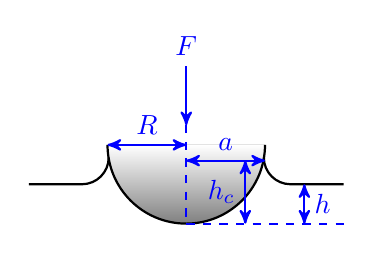
\begin{tikzpicture}
\fill[top color=white, bottom color=gray] (-1,0) arc(-180:0:1);
\draw[thick] (-1,0) arc(-180:0:1);
\draw[thick]  (-2,-0.5) -- (-1.325,-0.5) arc(-90:0:0.34);
\draw[thick]  (2,-0.5) -- (1.325,-0.5) arc(270:180:0.34);
\draw[thick,blue,dashed] (0,-1)--(2,-1) (0,0.25)--(0,-1);
\draw[thick,blue,<->,>=stealth'] (0,-0.2)--(1,-0.2) node[midway,above]{$a$};

\draw[thick,blue,<-,>=stealth'] (0,0.25)--(0,1) node[above]{$F$};
\draw[thick,blue,<->,>=stealth'] (0,0)--(-1,0) node[midway,above]{$R$};
\draw[thick,blue,<->,>=stealth'] (0.75,-1)--(0.75,-0.2) node[midway,left]{$h_c$};

\draw[thick,blue,<->,>=stealth'] (1.5,-1)--(1.5,-0.5) node[midway,right]{$h$};
\end{tikzpicture}
\end{center}
\end{minipage}
因为硬度$H$的定义为
\[
H = \frac{F}{\pi a^2}
, \quad\text{而}~
a = \sqrt{R^2 - (R-h_c)^2}
\]
所以$H$同样是上述自变量的函数, 即
\[
H = f_H(E, \nu; Y, n; h, R)
\]
选取$Y$和$R$作为基本量, 于是有
\[
%\frac{F}{Eh^2} = f_F \bigg(\nu; \frac{Y}{E}, n, \frac{R}{h}\bigg),\quad
%\frac{h_c}{h} = f_{h_c} \bigg(\nu; \frac{Y}{E}, n, \frac{R}{h}\bigg),\quad
\frac{H}{Y} = f_H\bigg(\frac{E}{Y},\nu, n, \frac{h}{R}\bigg)
\]
从上式可以看出$f_H$并不是常数, 只有当$E/Y\ll 1$且$h/R\ll 1$时, 才能近似的认为$H$与$Y$成正比. 但$h/R$并不满足$h/R\ll 1$, 且$h/R$随着$h$变化而变化, 因此, \textbf{不能断定硬度$H$和强度$Y$成正比}.
\end{solution}

\invisiblesubsection{什么是几何相似/相似律}
\begin{problem}[27]
什么是几何相似? 什么是几何相似律? 举例说明.
\end{problem}
% --------------------------------------------------------------------
\begin{solution}
\begin{itemize}
\item \textbf{几何相似}: 模型和原型的形状几何相似, 即模型和原型在任何几何维度上的长度比值相等, 即
\[
\bigg(\frac{l'}{l}, \frac{l''}{l},\cdots\bigg)_\mathrm{p} = \bigg(\frac{l'}{l}, \frac{l''}{l},\cdots\bigg)_\mathrm{m}
\]
\textbf{举例}: 例如在第\hyperref[problem:12]{12}题``\textcolor{blue}{能否用水洞做机翼的模型实验, 或用风洞做潜艇的模型实验?}''的结论中: 用水洞做机翼的模型实验, 或用风洞做潜艇的模型的必要条件之一就是几何相似:
$(l'/l,\cdots)_\mathrm{m}=(l'/l,\cdots)_\mathrm{p}$ 及 $\alpha_m = \alpha_p$.
\item \textbf{几何相似律}: 若模型采用与原型同样的材料($\alpha_E=1$且$\alpha_\nu=1$), 则在满足几何形状相似和分布函数相同的条件下, 在几何相似点
\[
\bigg(\frac{x}{l},\frac{y}{l},\frac{z}{l}\bigg)_\mathrm{p} 
=
\bigg(\frac{x}{l},\frac{y}{l},\frac{z}{l}\bigg)_\mathrm{m} 
\]
上, 有相同的相对位移, 应力和应变
\[
\bigg(\frac{w^i}{l}\bigg)_\mathrm{p} = \bigg(\frac{w^i}{l}\bigg)_\mathrm{m},~~
(\sigma_{ij})_\mathrm{p} = (\sigma_{ij})_\mathrm{m},~~
(\varepsilon_{ij})_\mathrm{p} = (\varepsilon_{ij})_\mathrm{m}
\]
\textbf{举例}: 例如在第\hyperref[problem:17]{17}题``\textcolor{blue}{讨论两端固定的梁在分布载荷作用下的挠度.}''的结论中: 只要保持$(q_m l^3/(EI))_\mathrm{p}=(q_m l^3/(EI))_\mathrm{m}$及$(l_q/l)_\mathrm{m}(l_q/l)_\mathrm{p}$, 就会有同一个无量纲挠度分布$w=lf(x/l)$.
\end{itemize}
\end{solution}

\invisiblesubsection{相似律是否一定要求几何相似}
\begin{problem}[28]
相似律是否一定要求几何相似? 为什么?
\end{problem}
% --------------------------------------------------------------------
\begin{solution}
相似律并不一定要求几何相似, 例如在第\hyperref[problem:19]{19}题``\textcolor{blue}{计论方形空心简支梁的挠度分布, 若用实心梁来模拟, 要求符合什么条件?}''的结论中: 不必要求模型的截面形状遵守几何相似的条件, 只要截面矩满足一定的条件, 便可用实心梁来模拟空心简支梁的挠度分布.
\end{solution}

\invisiblesubsection{典型金属中弹性变形和热传导的传播时间}
\begin{problem}[29]
估计和比较几种典型金属材料中弹性变形和热传导的传播时间.
\end{problem}
% --------------------------------------------------------------------
\begin{solution}
在谈庆明的专著\cite{tan_dimensional_2011}中, 式(5.14)和式(5.15)分别给出了弹性变形和热传导的传播的特征时间即
\[
t_{\mathrm{e.w.}} \approx \frac{l}{\sqrt{E/\rho}},\quad t_{\mathrm{h.c.}} \approx \frac{\rho c l^2}{\lambda}
\]
其中$l$为物体的特征长度, $E$和$\rho$分别为杨氏模量和密度, $c$和$\lambda$分别为比热和热导系数. 基于以上两式, 比较特征长度$l=1\mathrm{m}$的几种典型金属(铜, 钢, 铝)材料中弹性变形和热传导的传播时间, 见表\ref{tab:metaltime}. 
\begin{table}[!htb]
\centering
\caption{\label{tab:metaltime}几种典型金属材料(材料参数\cite{materialsproperty})中弹性变形和热传导的传播特征时间}
{\small
\begin{tabular}{c|cccc|cc|c}
\hline 
 & $\rho$ & $E$ & $c$ & $\lambda$ & $t_{\mathrm{e.w.}}$ & $t_{\mathrm{h.c.}}$ & \multirow{2}{*}{${\displaystyle O\bigg(\frac{t_{\mathrm{e.w.}}}{t_{\mathrm{h.c.}}}\bigg)}$}\tabularnewline
 & $10^{3}\mathrm{kg/m^{3}}$ & $10^{11}\mathrm{kg/s^{2}/m}$ & $10^{3}\mathrm{N\cdot m/kg/K}$ & $10^{2}\mathrm{N/s/K}$ & $10^{-4}\mathrm{s}$ & $10^{4}\mathrm{s}$ & \tabularnewline
\hline 
Cu & 8.90 & 1.17 & 0.386 & 3.93 & 2.76 & 0.87 & $10^{-8}$\tabularnewline
Fe & 7.90 & 2.00 & 0.470 & 0.329 & 1.99 & 11.29 & $10^{-9}$\tabularnewline
Al & 2.70 & 0.70 & 0.942 & 2.36 & 1.96 & 1.08 & $10^{-8}$\tabularnewline
\hline 
\end{tabular}}
\end{table}
由此可见, 常见金属材料的弹性变形和热传导的特征传播时间相差约八到九个量级. 由局部温升引起的应力和应变的变化极其迅速地传播到物体内部各处, 而热传导与其相比则十分缓慢. 可以近似地认为两种效应是可以解耦的.
\end{solution}

\invisiblesubsection{含水地层中弹性变形和渗流的传播时间}
\begin{problem}[30]
估计和比较含水地层中弹性变形和渗流的传播时间.
\end{problem}
% --------------------------------------------------------------------
\begin{solution}
由达西定律, 渗流的水力坡度与渗流流速的一次方成正比, 即渗流的流速
\[
v = kJ = -k \frac{dH}{ds}
\]
其中$k$为渗透系数, $J$为水力坡降. 因此渗流的传播的特征时间为
\[
t_\mathrm{i.f.} \approx \frac{l}{v}
\]
其中$l$为特征长度, 这里取$l=1\mathrm{m}$.  含水层的渗透系数为$100-0.001\mathrm{cm/s}$, 这里取$k=10^{-3}\mathrm{m/s}$, 水力陂度$J=1$, 杨氏模量为$E=10^9 \mathrm{Pa}$, 密度近似取水的密度$10^3\mathrm{kg/m^3}$. 以上参数的选取参考了\cite{basic_Hydrogeology, viera_mathematical_2012, wiki_hydraulic_conductivity}.则弹性变形和渗流的传播时间为
\[
t_\mathrm{e.w.} \approx \frac{l}{\sqrt{E/\rho}} = \frac{1\mathrm{m}}{\sqrt{10^9 \mathrm{Pa}/ 10^3\mathrm{kg/m^3}}} = 10^{-3} \mathrm{s},
\qquad
t_\mathrm{i.f.} \approx  \frac{l}{v} = \frac{1\mathrm{m}}{1\times10^{-3}\mathrm{m/s}} = 10^3 \mathrm{s}
\]
由此可见, 含水地层中弹性变形和渗流的传播时间相差约六个量级, 由局部渗流引起的应力和应变的变化极其迅速地传播到物体内部各处, 而渗流与其相比则十分缓慢. 可以近似地认为两种效应是可以解耦的\footnote{\textcolor{red}{谈老师批注: 若考虑土壤骨架变形, 分析会更复杂一些.} 由于时间关系, 有关土壤骨架变形的讨论, 本人暂未补充.}.
\end{solution}


\newpage

\noindent\textbf{注: 本文档是在本人量纲分析课程作业的基础上, 根据谈老师的批注及课上讨论修改补充而成. 部分课后习题的解答参考了夏伟光同学的量纲作业整理\cite{xiaweiguang}. 量纲分析是一门非常有用的课程, 而且谈庆明老师的课讲得非常好, 强列推荐同学们选这门课.}

\bibliographystyle{unsrt}
\bibliography{biblo}

\newpage
%\invisiblesection{近三年考试试题}
\appendix
\appendixpage
%\section{近三年考试试题}

\noindent\textbf{注: 这里给出了近三年的量纲分析考试题, 仅供后届同学平时练习和期末复习参考. 由试题可以看出, 谈老师的考题大多源于课堂和课后习题, 偏重基础和概念. 只要上课认真听讲, 作业认真做, 考试基本没有难度.}

\section{2012试题}
\begin{enumerate}
\item 怎样正确理解所谓``低速绕流''和所谓``高速冲击''的提法?
\item 请对单摆的周期做出正确又简炼的量纲分析.
\item 在两种液体中已知一种液体的粘性系数, 如何用一个小球来测定另一种液体的粘性系数?
\item 弹性波有哪几类? 对每一类弹性简谐波, 从物理上考虑, 可以用什么特征量来度量波长?
\end{enumerate}

\section{2013试题}

\begin{enumerate}
\item 对固体力学问题和流体力学问题, 各举两个无量纲数, 并说明将该数用在判据中的例子.
\item 物理问题中的因果关系是否应当由无量纲的形式? 说明理由, 并举例.
\item 对圆管流动来说, 决定总管阻和决定摩擦系数的自变量是否相同? 为什么?
\item 色散波和非色散波各举一例, 并说明发生色散现象的物理原因.
\end{enumerate}

\section{2014试题}
\begin{enumerate}
\item 一个家庭主妇和一个总理怎么样用量纲分析来管家和治国?
\item 对变形问题和流动问题分别给出两个无量纲数, 并说明物理意义和判据中的应用.
\item 说明用小球自由落体运动测定液体的粘性系数的原理.
\item 弹性波有哪几类? 从物理上考虑, 用什么量来度量简谐波的波长?
\end{enumerate}

\end{document} 
